\documentclass{slides}

\title[MCMC]{Mixture Models}
\author[Andrews]{Mark Andrews \& Thom Baguley}

\begin{document}
{
	\begin{frame}
		\titlepage
	\end{frame}
}


\begin{frame}
	\frametitle{Mixture models}
	\begin{itemize}

		\item Given a set of observed variables $y_1, y_2 \ldots y_n$,
			it is common to model them as distributed according to
			a parameteric density function density function
			$\Prob{y \given \theta}$ whose parameter $\theta$ are
			unknown.

		\item For example, we could model $y_1, y_2 \ldots y_n$ as 
			\[
				y_i \sim N(\mu, \sigma^2),\quad\text{for $i \in {1 \ldots n}$.}
			\]
		where $\mu$ and $\sigma$ are unknown.

	\item We could, however, models $y_1, y_2 \ldots y_n$ as distributed according to a finite \emph{mixture} of parametric density functions.
		For example, 
		\[
			y_i \sim \sum_{k=1}^K N(\mu_k, \sigma_k) \Prob{\mu_k, \sigma_k}, \quad\text{for $i \in {1 \ldots n}$.}
		\]
	

	\end{itemize}
	\end{frame}

	\begin{frame}
	\frametitle{Mixture Models}
	\noindent A mixture of Gaussians density function.
	\vspace{-2\baselineskip}
	\begin{center}
	
% Created by tikzDevice version 0.5.3 on 2011-03-10 19:24:09
\begin{tikzpicture}[x=1pt,y=1pt]
\draw[color=white,opacity=0] (0,0) rectangle (216.81,216.81);
\begin{scope}
\path[clip] ( 49.20, 61.20) rectangle (191.61,167.61);
\definecolor[named]{drawColor}{rgb}{0.13,0.02,0.33}
\definecolor[named]{drawColor}{rgb}{0.00,0.00,0.00}

\draw[color=drawColor,line cap=round,line join=round,fill opacity=0.00,] ( 54.47, 65.14) --
	( 54.61, 65.18) --
	( 54.74, 65.23) --
	( 54.87, 65.27) --
	( 55.00, 65.32) --
	( 55.13, 65.37) --
	( 55.27, 65.42) --
	( 55.40, 65.47) --
	( 55.53, 65.52) --
	( 55.66, 65.57) --
	( 55.79, 65.63) --
	( 55.93, 65.69) --
	( 56.06, 65.74) --
	( 56.19, 65.80) --
	( 56.32, 65.86) --
	( 56.45, 65.93) --
	( 56.59, 65.99) --
	( 56.72, 66.06) --
	( 56.85, 66.13) --
	( 56.98, 66.20) --
	( 57.11, 66.27) --
	( 57.25, 66.35) --
	( 57.38, 66.42) --
	( 57.51, 66.50) --
	( 57.64, 66.58) --
	( 57.77, 66.66) --
	( 57.91, 66.75) --
	( 58.04, 66.84) --
	( 58.17, 66.93) --
	( 58.30, 67.02) --
	( 58.43, 67.11) --
	( 58.57, 67.21) --
	( 58.70, 67.31) --
	( 58.83, 67.41) --
	( 58.96, 67.51) --
	( 59.09, 67.62) --
	( 59.23, 67.73) --
	( 59.36, 67.84) --
	( 59.49, 67.95) --
	( 59.62, 68.07) --
	( 59.75, 68.19) --
	( 59.89, 68.32) --
	( 60.02, 68.44) --
	( 60.15, 68.57) --
	( 60.28, 68.70) --
	( 60.41, 68.84) --
	( 60.55, 68.98) --
	( 60.68, 69.12) --
	( 60.81, 69.27) --
	( 60.94, 69.41) --
	( 61.07, 69.57) --
	( 61.21, 69.72) --
	( 61.34, 69.88) --
	( 61.47, 70.04) --
	( 61.60, 70.21) --
	( 61.73, 70.38) --
	( 61.87, 70.56) --
	( 62.00, 70.73) --
	( 62.13, 70.92) --
	( 62.26, 71.10) --
	( 62.39, 71.29) --
	( 62.53, 71.49) --
	( 62.66, 71.68) --
	( 62.79, 71.89) --
	( 62.92, 72.09) --
	( 63.05, 72.30) --
	( 63.19, 72.52) --
	( 63.32, 72.74) --
	( 63.45, 72.96) --
	( 63.58, 73.19) --
	( 63.71, 73.42) --
	( 63.85, 73.66) --
	( 63.98, 73.90) --
	( 64.11, 74.15) --
	( 64.24, 74.40) --
	( 64.37, 74.66) --
	( 64.51, 74.92) --
	( 64.64, 75.19) --
	( 64.77, 75.46) --
	( 64.90, 75.73) --
	( 65.03, 76.01) --
	( 65.17, 76.30) --
	( 65.30, 76.59) --
	( 65.43, 76.89) --
	( 65.56, 77.19) --
	( 65.69, 77.50) --
	( 65.83, 77.81) --
	( 65.96, 78.13) --
	( 66.09, 78.46) --
	( 66.22, 78.78) --
	( 66.35, 79.12) --
	( 66.49, 79.46) --
	( 66.62, 79.81) --
	( 66.75, 80.16) --
	( 66.88, 80.51) --
	( 67.01, 80.88) --
	( 67.15, 81.25) --
	( 67.28, 81.62) --
	( 67.41, 82.00) --
	( 67.54, 82.39) --
	( 67.67, 82.78) --
	( 67.81, 83.17) --
	( 67.94, 83.58) --
	( 68.07, 83.99) --
	( 68.20, 84.40) --
	( 68.33, 84.82) --
	( 68.47, 85.25) --
	( 68.60, 85.68) --
	( 68.73, 86.12) --
	( 68.86, 86.56) --
	( 68.99, 87.01) --
	( 69.13, 87.47) --
	( 69.26, 87.93) --
	( 69.39, 88.40) --
	( 69.52, 88.87) --
	( 69.65, 89.35) --
	( 69.79, 89.83) --
	( 69.92, 90.33) --
	( 70.05, 90.82) --
	( 70.18, 91.32) --
	( 70.31, 91.83) --
	( 70.45, 92.34) --
	( 70.58, 92.86) --
	( 70.71, 93.39) --
	( 70.84, 93.92) --
	( 70.97, 94.45) --
	( 71.11, 94.99) --
	( 71.24, 95.54) --
	( 71.37, 96.09) --
	( 71.50, 96.65) --
	( 71.63, 97.21) --
	( 71.77, 97.78) --
	( 71.90, 98.35) --
	( 72.03, 98.93) --
	( 72.16, 99.51) --
	( 72.29,100.10) --
	( 72.43,100.69) --
	( 72.56,101.29) --
	( 72.69,101.89) --
	( 72.82,102.50) --
	( 72.95,103.11) --
	( 73.09,103.72) --
	( 73.22,104.34) --
	( 73.35,104.96) --
	( 73.48,105.59) --
	( 73.61,106.22) --
	( 73.75,106.86) --
	( 73.88,107.50) --
	( 74.01,108.14) --
	( 74.14,108.79) --
	( 74.27,109.43) --
	( 74.41,110.09) --
	( 74.54,110.74) --
	( 74.67,111.40) --
	( 74.80,112.06) --
	( 74.93,112.73) --
	( 75.07,113.39) --
	( 75.20,114.06) --
	( 75.33,114.73) --
	( 75.46,115.41) --
	( 75.59,116.08) --
	( 75.73,116.76) --
	( 75.86,117.44) --
	( 75.99,118.12) --
	( 76.12,118.80) --
	( 76.25,119.48) --
	( 76.39,120.17) --
	( 76.52,120.85) --
	( 76.65,121.54) --
	( 76.78,122.22) --
	( 76.91,122.91) --
	( 77.05,123.60) --
	( 77.18,124.28) --
	( 77.31,124.97) --
	( 77.44,125.66) --
	( 77.57,126.34) --
	( 77.71,127.03) --
	( 77.84,127.71) --
	( 77.97,128.39) --
	( 78.10,129.07) --
	( 78.23,129.75) --
	( 78.37,130.43) --
	( 78.50,131.10) --
	( 78.63,131.78) --
	( 78.76,132.45) --
	( 78.89,133.12) --
	( 79.03,133.78) --
	( 79.16,134.45) --
	( 79.29,135.11) --
	( 79.42,135.76) --
	( 79.55,136.42) --
	( 79.69,137.07) --
	( 79.82,137.71) --
	( 79.95,138.35) --
	( 80.08,138.99) --
	( 80.21,139.62) --
	( 80.35,140.25) --
	( 80.48,140.88) --
	( 80.61,141.49) --
	( 80.74,142.11) --
	( 80.87,142.71) --
	( 81.01,143.32) --
	( 81.14,143.91) --
	( 81.27,144.50) --
	( 81.40,145.09) --
	( 81.53,145.67) --
	( 81.67,146.24) --
	( 81.80,146.80) --
	( 81.93,147.36) --
	( 82.06,147.91) --
	( 82.19,148.45) --
	( 82.32,148.99) --
	( 82.46,149.52) --
	( 82.59,150.04) --
	( 82.72,150.55) --
	( 82.85,151.06) --
	( 82.98,151.55) --
	( 83.12,152.04) --
	( 83.25,152.52) --
	( 83.38,152.99) --
	( 83.51,153.45) --
	( 83.64,153.91) --
	( 83.78,154.35) --
	( 83.91,154.79) --
	( 84.04,155.21) --
	( 84.17,155.63) --
	( 84.30,156.04) --
	( 84.44,156.43) --
	( 84.57,156.82) --
	( 84.70,157.20) --
	( 84.83,157.57) --
	( 84.96,157.92) --
	( 85.10,158.27) --
	( 85.23,158.61) --
	( 85.36,158.93) --
	( 85.49,159.25) --
	( 85.62,159.55) --
	( 85.76,159.85) --
	( 85.89,160.13) --
	( 86.02,160.41) --
	( 86.15,160.67) --
	( 86.28,160.92) --
	( 86.42,161.16) --
	( 86.55,161.39) --
	( 86.68,161.61) --
	( 86.81,161.82) --
	( 86.94,162.01) --
	( 87.08,162.20) --
	( 87.21,162.37) --
	( 87.34,162.54) --
	( 87.47,162.69) --
	( 87.60,162.83) --
	( 87.74,162.96) --
	( 87.87,163.08) --
	( 88.00,163.19) --
	( 88.13,163.29) --
	( 88.26,163.37) --
	( 88.40,163.45) --
	( 88.53,163.51) --
	( 88.66,163.56) --
	( 88.79,163.61) --
	( 88.92,163.64) --
	( 89.06,163.66) --
	( 89.19,163.67) --
	( 89.32,163.67) --
	( 89.45,163.66) --
	( 89.58,163.64) --
	( 89.72,163.60) --
	( 89.85,163.56) --
	( 89.98,163.51) --
	( 90.11,163.45) --
	( 90.24,163.37) --
	( 90.38,163.29) --
	( 90.51,163.20) --
	( 90.64,163.09) --
	( 90.77,162.98) --
	( 90.90,162.86) --
	( 91.04,162.73) --
	( 91.17,162.59) --
	( 91.30,162.44) --
	( 91.43,162.28) --
	( 91.56,162.11) --
	( 91.70,161.94) --
	( 91.83,161.75) --
	( 91.96,161.56) --
	( 92.09,161.36) --
	( 92.22,161.15) --
	( 92.36,160.93) --
	( 92.49,160.70) --
	( 92.62,160.47) --
	( 92.75,160.23) --
	( 92.88,159.98) --
	( 93.02,159.73) --
	( 93.15,159.47) --
	( 93.28,159.20) --
	( 93.41,158.92) --
	( 93.54,158.64) --
	( 93.68,158.35) --
	( 93.81,158.06) --
	( 93.94,157.76) --
	( 94.07,157.45) --
	( 94.20,157.14) --
	( 94.34,156.82) --
	( 94.47,156.50) --
	( 94.60,156.17) --
	( 94.73,155.84) --
	( 94.86,155.50) --
	( 95.00,155.16) --
	( 95.13,154.82) --
	( 95.26,154.47) --
	( 95.39,154.11) --
	( 95.52,153.76) --
	( 95.66,153.40) --
	( 95.79,153.03) --
	( 95.92,152.67) --
	( 96.05,152.30) --
	( 96.18,151.93) --
	( 96.32,151.55) --
	( 96.45,151.18) --
	( 96.58,150.80) --
	( 96.71,150.42) --
	( 96.84,150.03) --
	( 96.98,149.65) --
	( 97.11,149.26) --
	( 97.24,148.88) --
	( 97.37,148.49) --
	( 97.50,148.10) --
	( 97.64,147.71) --
	( 97.77,147.32) --
	( 97.90,146.93) --
	( 98.03,146.54) --
	( 98.16,146.16) --
	( 98.30,145.77) --
	( 98.43,145.38) --
	( 98.56,144.99) --
	( 98.69,144.60) --
	( 98.82,144.22) --
	( 98.96,143.83) --
	( 99.09,143.45) --
	( 99.22,143.06) --
	( 99.35,142.68) --
	( 99.48,142.30) --
	( 99.62,141.93) --
	( 99.75,141.55) --
	( 99.88,141.18) --
	(100.01,140.81) --
	(100.14,140.44) --
	(100.28,140.07) --
	(100.41,139.71) --
	(100.54,139.35) --
	(100.67,138.99) --
	(100.80,138.63) --
	(100.94,138.28) --
	(101.07,137.94) --
	(101.20,137.59) --
	(101.33,137.25) --
	(101.46,136.91) --
	(101.60,136.58) --
	(101.73,136.25) --
	(101.86,135.92) --
	(101.99,135.60) --
	(102.12,135.28) --
	(102.26,134.97) --
	(102.39,134.66) --
	(102.52,134.36) --
	(102.65,134.06) --
	(102.78,133.76) --
	(102.92,133.47) --
	(103.05,133.18) --
	(103.18,132.90) --
	(103.31,132.62) --
	(103.44,132.35) --
	(103.58,132.08) --
	(103.71,131.82) --
	(103.84,131.57) --
	(103.97,131.31) --
	(104.10,131.07) --
	(104.24,130.82) --
	(104.37,130.59) --
	(104.50,130.36) --
	(104.63,130.13) --
	(104.76,129.91) --
	(104.90,129.69) --
	(105.03,129.48) --
	(105.16,129.27) --
	(105.29,129.07) --
	(105.42,128.88) --
	(105.56,128.69) --
	(105.69,128.51) --
	(105.82,128.33) --
	(105.95,128.15) --
	(106.08,127.99) --
	(106.22,127.82) --
	(106.35,127.67) --
	(106.48,127.51) --
	(106.61,127.37) --
	(106.74,127.22) --
	(106.88,127.09) --
	(107.01,126.96) --
	(107.14,126.83) --
	(107.27,126.71) --
	(107.40,126.60) --
	(107.54,126.49) --
	(107.67,126.38) --
	(107.80,126.28) --
	(107.93,126.19) --
	(108.06,126.10) --
	(108.20,126.01) --
	(108.33,125.93) --
	(108.46,125.85) --
	(108.59,125.78) --
	(108.72,125.72) --
	(108.86,125.66) --
	(108.99,125.60) --
	(109.12,125.55) --
	(109.25,125.50) --
	(109.38,125.46) --
	(109.52,125.42) --
	(109.65,125.39) --
	(109.78,125.36) --
	(109.91,125.34) --
	(110.04,125.32) --
	(110.18,125.30) --
	(110.31,125.29) --
	(110.44,125.28) --
	(110.57,125.28) --
	(110.70,125.28) --
	(110.84,125.28) --
	(110.97,125.29) --
	(111.10,125.30) --
	(111.23,125.32) --
	(111.36,125.34) --
	(111.50,125.36) --
	(111.63,125.39) --
	(111.76,125.42) --
	(111.89,125.45) --
	(112.02,125.49) --
	(112.16,125.53) --
	(112.29,125.57) --
	(112.42,125.62) --
	(112.55,125.67) --
	(112.68,125.72) --
	(112.82,125.78) --
	(112.95,125.84) --
	(113.08,125.90) --
	(113.21,125.96) --
	(113.34,126.03) --
	(113.48,126.10) --
	(113.61,126.17) --
	(113.74,126.25) --
	(113.87,126.32) --
	(114.00,126.40) --
	(114.14,126.48) --
	(114.27,126.57) --
	(114.40,126.65) --
	(114.53,126.74) --
	(114.66,126.83) --
	(114.80,126.92) --
	(114.93,127.01) --
	(115.06,127.11) --
	(115.19,127.21) --
	(115.32,127.30) --
	(115.46,127.41) --
	(115.59,127.51) --
	(115.72,127.61) --
	(115.85,127.71) --
	(115.98,127.82) --
	(116.12,127.93) --
	(116.25,128.04) --
	(116.38,128.15) --
	(116.51,128.26) --
	(116.64,128.37) --
	(116.78,128.48) --
	(116.91,128.59) --
	(117.04,128.71) --
	(117.17,128.82) --
	(117.30,128.94) --
	(117.44,129.06) --
	(117.57,129.17) --
	(117.70,129.29) --
	(117.83,129.41) --
	(117.96,129.53) --
	(118.10,129.65) --
	(118.23,129.77) --
	(118.36,129.89) --
	(118.49,130.01) --
	(118.62,130.13) --
	(118.76,130.25) --
	(118.89,130.37) --
	(119.02,130.49) --
	(119.15,130.61) --
	(119.28,130.73) --
	(119.42,130.86) --
	(119.55,130.98) --
	(119.68,131.10) --
	(119.81,131.22) --
	(119.94,131.34) --
	(120.08,131.46) --
	(120.21,131.58) --
	(120.34,131.70) --
	(120.47,131.81) --
	(120.60,131.93) --
	(120.73,132.05) --
	(120.87,132.17) --
	(121.00,132.28) --
	(121.13,132.40) --
	(121.26,132.52) --
	(121.39,132.63) --
	(121.53,132.74) --
	(121.66,132.86) --
	(121.79,132.97) --
	(121.92,133.08) --
	(122.05,133.19) --
	(122.19,133.30) --
	(122.32,133.41) --
	(122.45,133.52) --
	(122.58,133.63) --
	(122.71,133.73) --
	(122.85,133.84) --
	(122.98,133.94) --
	(123.11,134.04) --
	(123.24,134.15) --
	(123.37,134.25) --
	(123.51,134.35) --
	(123.64,134.44) --
	(123.77,134.54) --
	(123.90,134.64) --
	(124.03,134.73) --
	(124.17,134.83) --
	(124.30,134.92) --
	(124.43,135.01) --
	(124.56,135.10) --
	(124.69,135.18) --
	(124.83,135.27) --
	(124.96,135.36) --
	(125.09,135.44) --
	(125.22,135.52) --
	(125.35,135.60) --
	(125.49,135.68) --
	(125.62,135.76) --
	(125.75,135.84) --
	(125.88,135.91) --
	(126.01,135.98) --
	(126.15,136.05) --
	(126.28,136.12) --
	(126.41,136.19) --
	(126.54,136.26) --
	(126.67,136.32) --
	(126.81,136.39) --
	(126.94,136.45) --
	(127.07,136.51) --
	(127.20,136.57) --
	(127.33,136.62) --
	(127.47,136.68) --
	(127.60,136.73) --
	(127.73,136.78) --
	(127.86,136.83) --
	(127.99,136.88) --
	(128.13,136.92) --
	(128.26,136.97) --
	(128.39,137.01) --
	(128.52,137.05) --
	(128.65,137.09) --
	(128.79,137.13) --
	(128.92,137.16) --
	(129.05,137.20) --
	(129.18,137.23) --
	(129.31,137.26) --
	(129.45,137.28) --
	(129.58,137.31) --
	(129.71,137.33) --
	(129.84,137.36) --
	(129.97,137.38) --
	(130.11,137.39) --
	(130.24,137.41) --
	(130.37,137.43) --
	(130.50,137.44) --
	(130.63,137.45) --
	(130.77,137.46) --
	(130.90,137.46) --
	(131.03,137.47) --
	(131.16,137.47) --
	(131.29,137.47) --
	(131.43,137.47) --
	(131.56,137.47) --
	(131.69,137.47) --
	(131.82,137.46) --
	(131.95,137.45) --
	(132.09,137.44) --
	(132.22,137.43) --
	(132.35,137.41) --
	(132.48,137.40) --
	(132.61,137.38) --
	(132.75,137.36) --
	(132.88,137.34) --
	(133.01,137.31) --
	(133.14,137.28) --
	(133.27,137.26) --
	(133.41,137.23) --
	(133.54,137.19) --
	(133.67,137.16) --
	(133.80,137.13) --
	(133.93,137.09) --
	(134.07,137.05) --
	(134.20,137.01) --
	(134.33,136.96) --
	(134.46,136.92) --
	(134.59,136.87) --
	(134.73,136.82) --
	(134.86,136.77) --
	(134.99,136.72) --
	(135.12,136.66) --
	(135.25,136.60) --
	(135.39,136.54) --
	(135.52,136.48) --
	(135.65,136.42) --
	(135.78,136.36) --
	(135.91,136.29) --
	(136.05,136.22) --
	(136.18,136.15) --
	(136.31,136.08) --
	(136.44,136.00) --
	(136.57,135.93) --
	(136.71,135.85) --
	(136.84,135.77) --
	(136.97,135.69) --
	(137.10,135.60) --
	(137.23,135.52) --
	(137.37,135.43) --
	(137.50,135.34) --
	(137.63,135.25) --
	(137.76,135.16) --
	(137.89,135.07) --
	(138.03,134.97) --
	(138.16,134.87) --
	(138.29,134.77) --
	(138.42,134.67) --
	(138.55,134.57) --
	(138.69,134.46) --
	(138.82,134.35) --
	(138.95,134.24) --
	(139.08,134.13) --
	(139.21,134.02) --
	(139.35,133.91) --
	(139.48,133.79) --
	(139.61,133.67) --
	(139.74,133.56) --
	(139.87,133.43) --
	(140.01,133.31) --
	(140.14,133.19) --
	(140.27,133.06) --
	(140.40,132.93) --
	(140.53,132.81) --
	(140.67,132.67) --
	(140.80,132.54) --
	(140.93,132.41) --
	(141.06,132.27) --
	(141.19,132.13) --
	(141.33,132.00) --
	(141.46,131.86) --
	(141.59,131.71) --
	(141.72,131.57) --
	(141.85,131.42) --
	(141.99,131.28) --
	(142.12,131.13) --
	(142.25,130.98) --
	(142.38,130.83) --
	(142.51,130.67) --
	(142.65,130.52) --
	(142.78,130.36) --
	(142.91,130.21) --
	(143.04,130.05) --
	(143.17,129.89) --
	(143.31,129.73) --
	(143.44,129.56) --
	(143.57,129.40) --
	(143.70,129.23) --
	(143.83,129.07) --
	(143.97,128.90) --
	(144.10,128.73) --
	(144.23,128.56) --
	(144.36,128.38) --
	(144.49,128.21) --
	(144.63,128.03) --
	(144.76,127.86) --
	(144.89,127.68) --
	(145.02,127.50) --
	(145.15,127.32) --
	(145.29,127.14) --
	(145.42,126.95) --
	(145.55,126.77) --
	(145.68,126.58) --
	(145.81,126.40) --
	(145.95,126.21) --
	(146.08,126.02) --
	(146.21,125.83) --
	(146.34,125.64) --
	(146.47,125.45) --
	(146.61,125.25) --
	(146.74,125.06) --
	(146.87,124.86) --
	(147.00,124.66) --
	(147.13,124.47) --
	(147.27,124.27) --
	(147.40,124.07) --
	(147.53,123.87) --
	(147.66,123.66) --
	(147.79,123.46) --
	(147.93,123.26) --
	(148.06,123.05) --
	(148.19,122.84) --
	(148.32,122.64) --
	(148.45,122.43) --
	(148.59,122.22) --
	(148.72,122.01) --
	(148.85,121.80) --
	(148.98,121.59) --
	(149.11,121.38) --
	(149.25,121.16) --
	(149.38,120.95) --
	(149.51,120.73) --
	(149.64,120.52) --
	(149.77,120.30) --
	(149.91,120.08) --
	(150.04,119.87) --
	(150.17,119.65) --
	(150.30,119.43) --
	(150.43,119.21) --
	(150.57,118.99) --
	(150.70,118.76) --
	(150.83,118.54) --
	(150.96,118.32) --
	(151.09,118.09) --
	(151.23,117.87) --
	(151.36,117.65) --
	(151.49,117.42) --
	(151.62,117.19) --
	(151.75,116.97) --
	(151.89,116.74) --
	(152.02,116.51) --
	(152.15,116.28) --
	(152.28,116.05) --
	(152.41,115.83) --
	(152.55,115.60) --
	(152.68,115.37) --
	(152.81,115.13) --
	(152.94,114.90) --
	(153.07,114.67) --
	(153.21,114.44) --
	(153.34,114.21) --
	(153.47,113.97) --
	(153.60,113.74) --
	(153.73,113.51) --
	(153.87,113.27) --
	(154.00,113.04) --
	(154.13,112.80) --
	(154.26,112.57) --
	(154.39,112.33) --
	(154.53,112.10) --
	(154.66,111.86) --
	(154.79,111.63) --
	(154.92,111.39) --
	(155.05,111.15) --
	(155.19,110.92) --
	(155.32,110.68) --
	(155.45,110.44) --
	(155.58,110.21) --
	(155.71,109.97) --
	(155.85,109.73) --
	(155.98,109.49) --
	(156.11,109.26) --
	(156.24,109.02) --
	(156.37,108.78) --
	(156.51,108.54) --
	(156.64,108.30) --
	(156.77,108.07) --
	(156.90,107.83) --
	(157.03,107.59) --
	(157.17,107.35) --
	(157.30,107.11) --
	(157.43,106.87) --
	(157.56,106.64) --
	(157.69,106.40) --
	(157.83,106.16) --
	(157.96,105.92) --
	(158.09,105.69) --
	(158.22,105.45) --
	(158.35,105.21) --
	(158.49,104.97) --
	(158.62,104.74) --
	(158.75,104.50) --
	(158.88,104.26) --
	(159.01,104.02) --
	(159.14,103.79) --
	(159.28,103.55) --
	(159.41,103.31) --
	(159.54,103.08) --
	(159.67,102.84) --
	(159.80,102.61) --
	(159.94,102.37) --
	(160.07,102.14) --
	(160.20,101.90) --
	(160.33,101.67) --
	(160.46,101.43) --
	(160.60,101.20) --
	(160.73,100.97) --
	(160.86,100.73) --
	(160.99,100.50) --
	(161.12,100.27) --
	(161.26,100.04) --
	(161.39, 99.81) --
	(161.52, 99.57) --
	(161.65, 99.34) --
	(161.78, 99.11) --
	(161.92, 98.88) --
	(162.05, 98.65) --
	(162.18, 98.42) --
	(162.31, 98.20) --
	(162.44, 97.97) --
	(162.58, 97.74) --
	(162.71, 97.51) --
	(162.84, 97.29) --
	(162.97, 97.06) --
	(163.10, 96.83) --
	(163.24, 96.61) --
	(163.37, 96.38) --
	(163.50, 96.16) --
	(163.63, 95.94) --
	(163.76, 95.71) --
	(163.90, 95.49) --
	(164.03, 95.27) --
	(164.16, 95.05) --
	(164.29, 94.83) --
	(164.42, 94.61) --
	(164.56, 94.39) --
	(164.69, 94.17) --
	(164.82, 93.95) --
	(164.95, 93.73) --
	(165.08, 93.52) --
	(165.22, 93.30) --
	(165.35, 93.08) --
	(165.48, 92.87) --
	(165.61, 92.66) --
	(165.74, 92.44) --
	(165.88, 92.23) --
	(166.01, 92.02) --
	(166.14, 91.81) --
	(166.27, 91.60) --
	(166.40, 91.39) --
	(166.54, 91.18) --
	(166.67, 90.97) --
	(166.80, 90.76) --
	(166.93, 90.55) --
	(167.06, 90.35) --
	(167.20, 90.14) --
	(167.33, 89.94) --
	(167.46, 89.73) --
	(167.59, 89.53) --
	(167.72, 89.33) --
	(167.86, 89.13) --
	(167.99, 88.92) --
	(168.12, 88.72) --
	(168.25, 88.53) --
	(168.38, 88.33) --
	(168.52, 88.13) --
	(168.65, 87.93) --
	(168.78, 87.74) --
	(168.91, 87.54) --
	(169.04, 87.35) --
	(169.18, 87.16) --
	(169.31, 86.96) --
	(169.44, 86.77) --
	(169.57, 86.58) --
	(169.70, 86.39) --
	(169.84, 86.20) --
	(169.97, 86.01) --
	(170.10, 85.83) --
	(170.23, 85.64) --
	(170.36, 85.45) --
	(170.50, 85.27) --
	(170.63, 85.09) --
	(170.76, 84.90) --
	(170.89, 84.72) --
	(171.02, 84.54) --
	(171.16, 84.36) --
	(171.29, 84.18) --
	(171.42, 84.00) --
	(171.55, 83.83) --
	(171.68, 83.65) --
	(171.82, 83.47) --
	(171.95, 83.30) --
	(172.08, 83.13) --
	(172.21, 82.95) --
	(172.34, 82.78) --
	(172.48, 82.61) --
	(172.61, 82.44) --
	(172.74, 82.27) --
	(172.87, 82.10) --
	(173.00, 81.94) --
	(173.14, 81.77) --
	(173.27, 81.60) --
	(173.40, 81.44) --
	(173.53, 81.28) --
	(173.66, 81.11) --
	(173.80, 80.95) --
	(173.93, 80.79) --
	(174.06, 80.63) --
	(174.19, 80.47) --
	(174.32, 80.32) --
	(174.46, 80.16) --
	(174.59, 80.00) --
	(174.72, 79.85) --
	(174.85, 79.70) --
	(174.98, 79.54) --
	(175.12, 79.39) --
	(175.25, 79.24) --
	(175.38, 79.09) --
	(175.51, 78.94) --
	(175.64, 78.79) --
	(175.78, 78.65) --
	(175.91, 78.50) --
	(176.04, 78.36) --
	(176.17, 78.21) --
	(176.30, 78.07) --
	(176.44, 77.93) --
	(176.57, 77.78) --
	(176.70, 77.64) --
	(176.83, 77.50) --
	(176.96, 77.37) --
	(177.10, 77.23) --
	(177.23, 77.09) --
	(177.36, 76.96) --
	(177.49, 76.82) --
	(177.62, 76.69) --
	(177.76, 76.56) --
	(177.89, 76.42) --
	(178.02, 76.29) --
	(178.15, 76.16) --
	(178.28, 76.03) --
	(178.42, 75.91) --
	(178.55, 75.78) --
	(178.68, 75.65) --
	(178.81, 75.53) --
	(178.94, 75.40) --
	(179.08, 75.28) --
	(179.21, 75.16) --
	(179.34, 75.04) --
	(179.47, 74.92) --
	(179.60, 74.80) --
	(179.74, 74.68) --
	(179.87, 74.56) --
	(180.00, 74.44) --
	(180.13, 74.33) --
	(180.26, 74.21) --
	(180.40, 74.10) --
	(180.53, 73.98) --
	(180.66, 73.87) --
	(180.79, 73.76) --
	(180.92, 73.65) --
	(181.06, 73.54) --
	(181.19, 73.43) --
	(181.32, 73.32) --
	(181.45, 73.22) --
	(181.58, 73.11) --
	(181.72, 73.01) --
	(181.85, 72.90) --
	(181.98, 72.80) --
	(182.11, 72.70) --
	(182.24, 72.59) --
	(182.38, 72.49) --
	(182.51, 72.39) --
	(182.64, 72.29) --
	(182.77, 72.20) --
	(182.90, 72.10) --
	(183.04, 72.00) --
	(183.17, 71.91) --
	(183.30, 71.81) --
	(183.43, 71.72) --
	(183.56, 71.62) --
	(183.70, 71.53) --
	(183.83, 71.44) --
	(183.96, 71.35) --
	(184.09, 71.26) --
	(184.22, 71.17) --
	(184.36, 71.08) --
	(184.49, 70.99) --
	(184.62, 70.91) --
	(184.75, 70.82) --
	(184.88, 70.74) --
	(185.02, 70.65) --
	(185.15, 70.57) --
	(185.28, 70.49) --
	(185.41, 70.40) --
	(185.54, 70.32) --
	(185.68, 70.24) --
	(185.81, 70.16) --
	(185.94, 70.08) --
	(186.07, 70.01) --
	(186.20, 69.93) --
	(186.34, 69.85);
\end{scope}
\begin{scope}
\path[clip] (  0.00,  0.00) rectangle (216.81,216.81);
\definecolor[named]{drawColor}{rgb}{0.13,0.02,0.33}
\definecolor[named]{drawColor}{rgb}{0.00,0.00,0.00}

\draw[color=drawColor,line cap=round,line join=round,fill opacity=0.00,] ( 54.47, 61.20) -- (186.34, 61.20);

\draw[color=drawColor,line cap=round,line join=round,fill opacity=0.00,] ( 54.47, 61.20) -- ( 54.47, 55.20);

\draw[color=drawColor,line cap=round,line join=round,fill opacity=0.00,] ( 76.45, 61.20) -- ( 76.45, 55.20);

\draw[color=drawColor,line cap=round,line join=round,fill opacity=0.00,] ( 98.43, 61.20) -- ( 98.43, 55.20);

\draw[color=drawColor,line cap=round,line join=round,fill opacity=0.00,] (120.41, 61.20) -- (120.41, 55.20);

\draw[color=drawColor,line cap=round,line join=round,fill opacity=0.00,] (142.38, 61.20) -- (142.38, 55.20);

\draw[color=drawColor,line cap=round,line join=round,fill opacity=0.00,] (164.36, 61.20) -- (164.36, 55.20);

\draw[color=drawColor,line cap=round,line join=round,fill opacity=0.00,] (186.34, 61.20) -- (186.34, 55.20);

\node[color=drawColor,anchor=base,inner sep=0pt, outer sep=0pt, scale=  1.00] at ( 54.47, 37.20) {-6%
};

\node[color=drawColor,anchor=base,inner sep=0pt, outer sep=0pt, scale=  1.00] at ( 76.45, 37.20) {-4%
};

\node[color=drawColor,anchor=base,inner sep=0pt, outer sep=0pt, scale=  1.00] at ( 98.43, 37.20) {-2%
};

\node[color=drawColor,anchor=base,inner sep=0pt, outer sep=0pt, scale=  1.00] at (120.41, 37.20) {0%
};

\node[color=drawColor,anchor=base,inner sep=0pt, outer sep=0pt, scale=  1.00] at (142.38, 37.20) {2%
};

\node[color=drawColor,anchor=base,inner sep=0pt, outer sep=0pt, scale=  1.00] at (164.36, 37.20) {4%
};

\node[color=drawColor,anchor=base,inner sep=0pt, outer sep=0pt, scale=  1.00] at (186.34, 37.20) {6%
};

\draw[color=drawColor,line cap=round,line join=round,fill opacity=0.00,] ( 49.20, 63.74) -- ( 49.20,157.95);

\draw[color=drawColor,line cap=round,line join=round,fill opacity=0.00,] ( 49.20, 63.74) -- ( 43.20, 63.74);

\draw[color=drawColor,line cap=round,line join=round,fill opacity=0.00,] ( 49.20, 95.14) -- ( 43.20, 95.14);

\draw[color=drawColor,line cap=round,line join=round,fill opacity=0.00,] ( 49.20,126.54) -- ( 43.20,126.54);

\draw[color=drawColor,line cap=round,line join=round,fill opacity=0.00,] ( 49.20,157.95) -- ( 43.20,157.95);

\node[rotate= 90.00,color=drawColor,anchor=base,inner sep=0pt, outer sep=0pt, scale=  1.00] at ( 37.20, 63.74) {0.00%
};

\node[rotate= 90.00,color=drawColor,anchor=base,inner sep=0pt, outer sep=0pt, scale=  1.00] at ( 37.20, 95.14) {0.05%
};

\node[rotate= 90.00,color=drawColor,anchor=base,inner sep=0pt, outer sep=0pt, scale=  1.00] at ( 37.20,126.54) {0.10%
};

\node[rotate= 90.00,color=drawColor,anchor=base,inner sep=0pt, outer sep=0pt, scale=  1.00] at ( 37.20,157.95) {0.15%
};

\draw[color=drawColor,line cap=round,line join=round,fill opacity=0.00,] ( 49.20, 61.20) --
	(191.61, 61.20) --
	(191.61,167.61) --
	( 49.20,167.61) --
	( 49.20, 61.20);
\end{scope}
\begin{scope}
\path[clip] (  0.00,  0.00) rectangle (216.81,216.81);
\definecolor[named]{drawColor}{rgb}{0.13,0.02,0.33}
\definecolor[named]{drawColor}{rgb}{0.00,0.00,0.00}

\node[color=drawColor,anchor=base,inner sep=0pt, outer sep=0pt, scale=  1.00] at (120.41, 13.20) {$y$
};

\node[rotate= 00.00,color=drawColor,anchor=base,inner sep=0pt, outer sep=0pt, scale=  1.00] at ( 13.20,114.41) {$\Prob{y}$
};
\end{scope}
\end{tikzpicture}

	\end{center}
	\end{frame}

	\begin{frame}
	\frametitle{Mixture Models}
	\noindent A mixture of Gaussians density function with component distributions shown in red.
	\vspace{-2\baselineskip}
	\begin{center}
	
% Created by tikzDevice version 0.5.3 on 2011-03-10 19:27:22
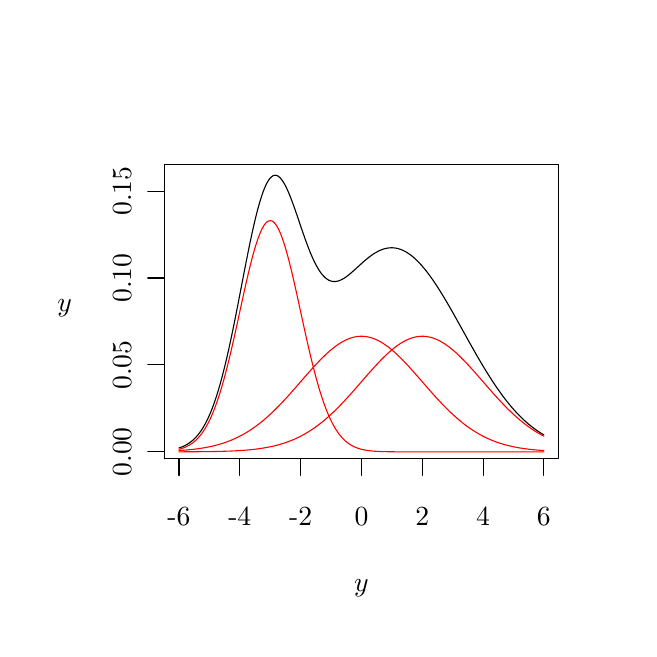
\begin{tikzpicture}[x=1pt,y=1pt]
\draw[color=white,opacity=0] (0,0) rectangle (216.81,216.81);
\begin{scope}
\path[clip] ( 49.20, 61.20) rectangle (191.61,167.61);
\definecolor[named]{drawColor}{rgb}{0.88,0.96,0.96}
\definecolor[named]{drawColor}{rgb}{0.00,0.00,0.00}

\draw[color=drawColor,line cap=round,line join=round,fill opacity=0.00,] ( 54.47, 65.14) --
	( 54.61, 65.18) --
	( 54.74, 65.23) --
	( 54.87, 65.27) --
	( 55.00, 65.32) --
	( 55.13, 65.37) --
	( 55.27, 65.42) --
	( 55.40, 65.47) --
	( 55.53, 65.52) --
	( 55.66, 65.57) --
	( 55.79, 65.63) --
	( 55.93, 65.69) --
	( 56.06, 65.74) --
	( 56.19, 65.80) --
	( 56.32, 65.86) --
	( 56.45, 65.93) --
	( 56.59, 65.99) --
	( 56.72, 66.06) --
	( 56.85, 66.13) --
	( 56.98, 66.20) --
	( 57.11, 66.27) --
	( 57.25, 66.35) --
	( 57.38, 66.42) --
	( 57.51, 66.50) --
	( 57.64, 66.58) --
	( 57.77, 66.66) --
	( 57.91, 66.75) --
	( 58.04, 66.84) --
	( 58.17, 66.93) --
	( 58.30, 67.02) --
	( 58.43, 67.11) --
	( 58.57, 67.21) --
	( 58.70, 67.31) --
	( 58.83, 67.41) --
	( 58.96, 67.51) --
	( 59.09, 67.62) --
	( 59.23, 67.73) --
	( 59.36, 67.84) --
	( 59.49, 67.95) --
	( 59.62, 68.07) --
	( 59.75, 68.19) --
	( 59.89, 68.32) --
	( 60.02, 68.44) --
	( 60.15, 68.57) --
	( 60.28, 68.70) --
	( 60.41, 68.84) --
	( 60.55, 68.98) --
	( 60.68, 69.12) --
	( 60.81, 69.27) --
	( 60.94, 69.41) --
	( 61.07, 69.57) --
	( 61.21, 69.72) --
	( 61.34, 69.88) --
	( 61.47, 70.04) --
	( 61.60, 70.21) --
	( 61.73, 70.38) --
	( 61.87, 70.56) --
	( 62.00, 70.73) --
	( 62.13, 70.92) --
	( 62.26, 71.10) --
	( 62.39, 71.29) --
	( 62.53, 71.49) --
	( 62.66, 71.68) --
	( 62.79, 71.89) --
	( 62.92, 72.09) --
	( 63.05, 72.30) --
	( 63.19, 72.52) --
	( 63.32, 72.74) --
	( 63.45, 72.96) --
	( 63.58, 73.19) --
	( 63.71, 73.42) --
	( 63.85, 73.66) --
	( 63.98, 73.90) --
	( 64.11, 74.15) --
	( 64.24, 74.40) --
	( 64.37, 74.66) --
	( 64.51, 74.92) --
	( 64.64, 75.19) --
	( 64.77, 75.46) --
	( 64.90, 75.73) --
	( 65.03, 76.01) --
	( 65.17, 76.30) --
	( 65.30, 76.59) --
	( 65.43, 76.89) --
	( 65.56, 77.19) --
	( 65.69, 77.50) --
	( 65.83, 77.81) --
	( 65.96, 78.13) --
	( 66.09, 78.46) --
	( 66.22, 78.78) --
	( 66.35, 79.12) --
	( 66.49, 79.46) --
	( 66.62, 79.81) --
	( 66.75, 80.16) --
	( 66.88, 80.51) --
	( 67.01, 80.88) --
	( 67.15, 81.25) --
	( 67.28, 81.62) --
	( 67.41, 82.00) --
	( 67.54, 82.39) --
	( 67.67, 82.78) --
	( 67.81, 83.17) --
	( 67.94, 83.58) --
	( 68.07, 83.99) --
	( 68.20, 84.40) --
	( 68.33, 84.82) --
	( 68.47, 85.25) --
	( 68.60, 85.68) --
	( 68.73, 86.12) --
	( 68.86, 86.56) --
	( 68.99, 87.01) --
	( 69.13, 87.47) --
	( 69.26, 87.93) --
	( 69.39, 88.40) --
	( 69.52, 88.87) --
	( 69.65, 89.35) --
	( 69.79, 89.83) --
	( 69.92, 90.33) --
	( 70.05, 90.82) --
	( 70.18, 91.32) --
	( 70.31, 91.83) --
	( 70.45, 92.34) --
	( 70.58, 92.86) --
	( 70.71, 93.39) --
	( 70.84, 93.92) --
	( 70.97, 94.45) --
	( 71.11, 94.99) --
	( 71.24, 95.54) --
	( 71.37, 96.09) --
	( 71.50, 96.65) --
	( 71.63, 97.21) --
	( 71.77, 97.78) --
	( 71.90, 98.35) --
	( 72.03, 98.93) --
	( 72.16, 99.51) --
	( 72.29,100.10) --
	( 72.43,100.69) --
	( 72.56,101.29) --
	( 72.69,101.89) --
	( 72.82,102.50) --
	( 72.95,103.11) --
	( 73.09,103.72) --
	( 73.22,104.34) --
	( 73.35,104.96) --
	( 73.48,105.59) --
	( 73.61,106.22) --
	( 73.75,106.86) --
	( 73.88,107.50) --
	( 74.01,108.14) --
	( 74.14,108.79) --
	( 74.27,109.43) --
	( 74.41,110.09) --
	( 74.54,110.74) --
	( 74.67,111.40) --
	( 74.80,112.06) --
	( 74.93,112.73) --
	( 75.07,113.39) --
	( 75.20,114.06) --
	( 75.33,114.73) --
	( 75.46,115.41) --
	( 75.59,116.08) --
	( 75.73,116.76) --
	( 75.86,117.44) --
	( 75.99,118.12) --
	( 76.12,118.80) --
	( 76.25,119.48) --
	( 76.39,120.17) --
	( 76.52,120.85) --
	( 76.65,121.54) --
	( 76.78,122.22) --
	( 76.91,122.91) --
	( 77.05,123.60) --
	( 77.18,124.28) --
	( 77.31,124.97) --
	( 77.44,125.66) --
	( 77.57,126.34) --
	( 77.71,127.03) --
	( 77.84,127.71) --
	( 77.97,128.39) --
	( 78.10,129.07) --
	( 78.23,129.75) --
	( 78.37,130.43) --
	( 78.50,131.10) --
	( 78.63,131.78) --
	( 78.76,132.45) --
	( 78.89,133.12) --
	( 79.03,133.78) --
	( 79.16,134.45) --
	( 79.29,135.11) --
	( 79.42,135.76) --
	( 79.55,136.42) --
	( 79.69,137.07) --
	( 79.82,137.71) --
	( 79.95,138.35) --
	( 80.08,138.99) --
	( 80.21,139.62) --
	( 80.35,140.25) --
	( 80.48,140.88) --
	( 80.61,141.49) --
	( 80.74,142.11) --
	( 80.87,142.71) --
	( 81.01,143.32) --
	( 81.14,143.91) --
	( 81.27,144.50) --
	( 81.40,145.09) --
	( 81.53,145.67) --
	( 81.67,146.24) --
	( 81.80,146.80) --
	( 81.93,147.36) --
	( 82.06,147.91) --
	( 82.19,148.45) --
	( 82.32,148.99) --
	( 82.46,149.52) --
	( 82.59,150.04) --
	( 82.72,150.55) --
	( 82.85,151.06) --
	( 82.98,151.55) --
	( 83.12,152.04) --
	( 83.25,152.52) --
	( 83.38,152.99) --
	( 83.51,153.45) --
	( 83.64,153.91) --
	( 83.78,154.35) --
	( 83.91,154.79) --
	( 84.04,155.21) --
	( 84.17,155.63) --
	( 84.30,156.04) --
	( 84.44,156.43) --
	( 84.57,156.82) --
	( 84.70,157.20) --
	( 84.83,157.57) --
	( 84.96,157.92) --
	( 85.10,158.27) --
	( 85.23,158.61) --
	( 85.36,158.93) --
	( 85.49,159.25) --
	( 85.62,159.55) --
	( 85.76,159.85) --
	( 85.89,160.13) --
	( 86.02,160.41) --
	( 86.15,160.67) --
	( 86.28,160.92) --
	( 86.42,161.16) --
	( 86.55,161.39) --
	( 86.68,161.61) --
	( 86.81,161.82) --
	( 86.94,162.01) --
	( 87.08,162.20) --
	( 87.21,162.37) --
	( 87.34,162.54) --
	( 87.47,162.69) --
	( 87.60,162.83) --
	( 87.74,162.96) --
	( 87.87,163.08) --
	( 88.00,163.19) --
	( 88.13,163.29) --
	( 88.26,163.37) --
	( 88.40,163.45) --
	( 88.53,163.51) --
	( 88.66,163.56) --
	( 88.79,163.61) --
	( 88.92,163.64) --
	( 89.06,163.66) --
	( 89.19,163.67) --
	( 89.32,163.67) --
	( 89.45,163.66) --
	( 89.58,163.64) --
	( 89.72,163.60) --
	( 89.85,163.56) --
	( 89.98,163.51) --
	( 90.11,163.45) --
	( 90.24,163.37) --
	( 90.38,163.29) --
	( 90.51,163.20) --
	( 90.64,163.09) --
	( 90.77,162.98) --
	( 90.90,162.86) --
	( 91.04,162.73) --
	( 91.17,162.59) --
	( 91.30,162.44) --
	( 91.43,162.28) --
	( 91.56,162.11) --
	( 91.70,161.94) --
	( 91.83,161.75) --
	( 91.96,161.56) --
	( 92.09,161.36) --
	( 92.22,161.15) --
	( 92.36,160.93) --
	( 92.49,160.70) --
	( 92.62,160.47) --
	( 92.75,160.23) --
	( 92.88,159.98) --
	( 93.02,159.73) --
	( 93.15,159.47) --
	( 93.28,159.20) --
	( 93.41,158.92) --
	( 93.54,158.64) --
	( 93.68,158.35) --
	( 93.81,158.06) --
	( 93.94,157.76) --
	( 94.07,157.45) --
	( 94.20,157.14) --
	( 94.34,156.82) --
	( 94.47,156.50) --
	( 94.60,156.17) --
	( 94.73,155.84) --
	( 94.86,155.50) --
	( 95.00,155.16) --
	( 95.13,154.82) --
	( 95.26,154.47) --
	( 95.39,154.11) --
	( 95.52,153.76) --
	( 95.66,153.40) --
	( 95.79,153.03) --
	( 95.92,152.67) --
	( 96.05,152.30) --
	( 96.18,151.93) --
	( 96.32,151.55) --
	( 96.45,151.18) --
	( 96.58,150.80) --
	( 96.71,150.42) --
	( 96.84,150.03) --
	( 96.98,149.65) --
	( 97.11,149.26) --
	( 97.24,148.88) --
	( 97.37,148.49) --
	( 97.50,148.10) --
	( 97.64,147.71) --
	( 97.77,147.32) --
	( 97.90,146.93) --
	( 98.03,146.54) --
	( 98.16,146.16) --
	( 98.30,145.77) --
	( 98.43,145.38) --
	( 98.56,144.99) --
	( 98.69,144.60) --
	( 98.82,144.22) --
	( 98.96,143.83) --
	( 99.09,143.45) --
	( 99.22,143.06) --
	( 99.35,142.68) --
	( 99.48,142.30) --
	( 99.62,141.93) --
	( 99.75,141.55) --
	( 99.88,141.18) --
	(100.01,140.81) --
	(100.14,140.44) --
	(100.28,140.07) --
	(100.41,139.71) --
	(100.54,139.35) --
	(100.67,138.99) --
	(100.80,138.63) --
	(100.94,138.28) --
	(101.07,137.94) --
	(101.20,137.59) --
	(101.33,137.25) --
	(101.46,136.91) --
	(101.60,136.58) --
	(101.73,136.25) --
	(101.86,135.92) --
	(101.99,135.60) --
	(102.12,135.28) --
	(102.26,134.97) --
	(102.39,134.66) --
	(102.52,134.36) --
	(102.65,134.06) --
	(102.78,133.76) --
	(102.92,133.47) --
	(103.05,133.18) --
	(103.18,132.90) --
	(103.31,132.62) --
	(103.44,132.35) --
	(103.58,132.08) --
	(103.71,131.82) --
	(103.84,131.57) --
	(103.97,131.31) --
	(104.10,131.07) --
	(104.24,130.82) --
	(104.37,130.59) --
	(104.50,130.36) --
	(104.63,130.13) --
	(104.76,129.91) --
	(104.90,129.69) --
	(105.03,129.48) --
	(105.16,129.27) --
	(105.29,129.07) --
	(105.42,128.88) --
	(105.56,128.69) --
	(105.69,128.51) --
	(105.82,128.33) --
	(105.95,128.15) --
	(106.08,127.99) --
	(106.22,127.82) --
	(106.35,127.67) --
	(106.48,127.51) --
	(106.61,127.37) --
	(106.74,127.22) --
	(106.88,127.09) --
	(107.01,126.96) --
	(107.14,126.83) --
	(107.27,126.71) --
	(107.40,126.60) --
	(107.54,126.49) --
	(107.67,126.38) --
	(107.80,126.28) --
	(107.93,126.19) --
	(108.06,126.10) --
	(108.20,126.01) --
	(108.33,125.93) --
	(108.46,125.85) --
	(108.59,125.78) --
	(108.72,125.72) --
	(108.86,125.66) --
	(108.99,125.60) --
	(109.12,125.55) --
	(109.25,125.50) --
	(109.38,125.46) --
	(109.52,125.42) --
	(109.65,125.39) --
	(109.78,125.36) --
	(109.91,125.34) --
	(110.04,125.32) --
	(110.18,125.30) --
	(110.31,125.29) --
	(110.44,125.28) --
	(110.57,125.28) --
	(110.70,125.28) --
	(110.84,125.28) --
	(110.97,125.29) --
	(111.10,125.30) --
	(111.23,125.32) --
	(111.36,125.34) --
	(111.50,125.36) --
	(111.63,125.39) --
	(111.76,125.42) --
	(111.89,125.45) --
	(112.02,125.49) --
	(112.16,125.53) --
	(112.29,125.57) --
	(112.42,125.62) --
	(112.55,125.67) --
	(112.68,125.72) --
	(112.82,125.78) --
	(112.95,125.84) --
	(113.08,125.90) --
	(113.21,125.96) --
	(113.34,126.03) --
	(113.48,126.10) --
	(113.61,126.17) --
	(113.74,126.25) --
	(113.87,126.32) --
	(114.00,126.40) --
	(114.14,126.48) --
	(114.27,126.57) --
	(114.40,126.65) --
	(114.53,126.74) --
	(114.66,126.83) --
	(114.80,126.92) --
	(114.93,127.01) --
	(115.06,127.11) --
	(115.19,127.21) --
	(115.32,127.30) --
	(115.46,127.41) --
	(115.59,127.51) --
	(115.72,127.61) --
	(115.85,127.71) --
	(115.98,127.82) --
	(116.12,127.93) --
	(116.25,128.04) --
	(116.38,128.15) --
	(116.51,128.26) --
	(116.64,128.37) --
	(116.78,128.48) --
	(116.91,128.59) --
	(117.04,128.71) --
	(117.17,128.82) --
	(117.30,128.94) --
	(117.44,129.06) --
	(117.57,129.17) --
	(117.70,129.29) --
	(117.83,129.41) --
	(117.96,129.53) --
	(118.10,129.65) --
	(118.23,129.77) --
	(118.36,129.89) --
	(118.49,130.01) --
	(118.62,130.13) --
	(118.76,130.25) --
	(118.89,130.37) --
	(119.02,130.49) --
	(119.15,130.61) --
	(119.28,130.73) --
	(119.42,130.86) --
	(119.55,130.98) --
	(119.68,131.10) --
	(119.81,131.22) --
	(119.94,131.34) --
	(120.08,131.46) --
	(120.21,131.58) --
	(120.34,131.70) --
	(120.47,131.81) --
	(120.60,131.93) --
	(120.73,132.05) --
	(120.87,132.17) --
	(121.00,132.28) --
	(121.13,132.40) --
	(121.26,132.52) --
	(121.39,132.63) --
	(121.53,132.74) --
	(121.66,132.86) --
	(121.79,132.97) --
	(121.92,133.08) --
	(122.05,133.19) --
	(122.19,133.30) --
	(122.32,133.41) --
	(122.45,133.52) --
	(122.58,133.63) --
	(122.71,133.73) --
	(122.85,133.84) --
	(122.98,133.94) --
	(123.11,134.04) --
	(123.24,134.15) --
	(123.37,134.25) --
	(123.51,134.35) --
	(123.64,134.44) --
	(123.77,134.54) --
	(123.90,134.64) --
	(124.03,134.73) --
	(124.17,134.83) --
	(124.30,134.92) --
	(124.43,135.01) --
	(124.56,135.10) --
	(124.69,135.18) --
	(124.83,135.27) --
	(124.96,135.36) --
	(125.09,135.44) --
	(125.22,135.52) --
	(125.35,135.60) --
	(125.49,135.68) --
	(125.62,135.76) --
	(125.75,135.84) --
	(125.88,135.91) --
	(126.01,135.98) --
	(126.15,136.05) --
	(126.28,136.12) --
	(126.41,136.19) --
	(126.54,136.26) --
	(126.67,136.32) --
	(126.81,136.39) --
	(126.94,136.45) --
	(127.07,136.51) --
	(127.20,136.57) --
	(127.33,136.62) --
	(127.47,136.68) --
	(127.60,136.73) --
	(127.73,136.78) --
	(127.86,136.83) --
	(127.99,136.88) --
	(128.13,136.92) --
	(128.26,136.97) --
	(128.39,137.01) --
	(128.52,137.05) --
	(128.65,137.09) --
	(128.79,137.13) --
	(128.92,137.16) --
	(129.05,137.20) --
	(129.18,137.23) --
	(129.31,137.26) --
	(129.45,137.28) --
	(129.58,137.31) --
	(129.71,137.33) --
	(129.84,137.36) --
	(129.97,137.38) --
	(130.11,137.39) --
	(130.24,137.41) --
	(130.37,137.43) --
	(130.50,137.44) --
	(130.63,137.45) --
	(130.77,137.46) --
	(130.90,137.46) --
	(131.03,137.47) --
	(131.16,137.47) --
	(131.29,137.47) --
	(131.43,137.47) --
	(131.56,137.47) --
	(131.69,137.47) --
	(131.82,137.46) --
	(131.95,137.45) --
	(132.09,137.44) --
	(132.22,137.43) --
	(132.35,137.41) --
	(132.48,137.40) --
	(132.61,137.38) --
	(132.75,137.36) --
	(132.88,137.34) --
	(133.01,137.31) --
	(133.14,137.28) --
	(133.27,137.26) --
	(133.41,137.23) --
	(133.54,137.19) --
	(133.67,137.16) --
	(133.80,137.13) --
	(133.93,137.09) --
	(134.07,137.05) --
	(134.20,137.01) --
	(134.33,136.96) --
	(134.46,136.92) --
	(134.59,136.87) --
	(134.73,136.82) --
	(134.86,136.77) --
	(134.99,136.72) --
	(135.12,136.66) --
	(135.25,136.60) --
	(135.39,136.54) --
	(135.52,136.48) --
	(135.65,136.42) --
	(135.78,136.36) --
	(135.91,136.29) --
	(136.05,136.22) --
	(136.18,136.15) --
	(136.31,136.08) --
	(136.44,136.00) --
	(136.57,135.93) --
	(136.71,135.85) --
	(136.84,135.77) --
	(136.97,135.69) --
	(137.10,135.60) --
	(137.23,135.52) --
	(137.37,135.43) --
	(137.50,135.34) --
	(137.63,135.25) --
	(137.76,135.16) --
	(137.89,135.07) --
	(138.03,134.97) --
	(138.16,134.87) --
	(138.29,134.77) --
	(138.42,134.67) --
	(138.55,134.57) --
	(138.69,134.46) --
	(138.82,134.35) --
	(138.95,134.24) --
	(139.08,134.13) --
	(139.21,134.02) --
	(139.35,133.91) --
	(139.48,133.79) --
	(139.61,133.67) --
	(139.74,133.56) --
	(139.87,133.43) --
	(140.01,133.31) --
	(140.14,133.19) --
	(140.27,133.06) --
	(140.40,132.93) --
	(140.53,132.81) --
	(140.67,132.67) --
	(140.80,132.54) --
	(140.93,132.41) --
	(141.06,132.27) --
	(141.19,132.13) --
	(141.33,132.00) --
	(141.46,131.86) --
	(141.59,131.71) --
	(141.72,131.57) --
	(141.85,131.42) --
	(141.99,131.28) --
	(142.12,131.13) --
	(142.25,130.98) --
	(142.38,130.83) --
	(142.51,130.67) --
	(142.65,130.52) --
	(142.78,130.36) --
	(142.91,130.21) --
	(143.04,130.05) --
	(143.17,129.89) --
	(143.31,129.73) --
	(143.44,129.56) --
	(143.57,129.40) --
	(143.70,129.23) --
	(143.83,129.07) --
	(143.97,128.90) --
	(144.10,128.73) --
	(144.23,128.56) --
	(144.36,128.38) --
	(144.49,128.21) --
	(144.63,128.03) --
	(144.76,127.86) --
	(144.89,127.68) --
	(145.02,127.50) --
	(145.15,127.32) --
	(145.29,127.14) --
	(145.42,126.95) --
	(145.55,126.77) --
	(145.68,126.58) --
	(145.81,126.40) --
	(145.95,126.21) --
	(146.08,126.02) --
	(146.21,125.83) --
	(146.34,125.64) --
	(146.47,125.45) --
	(146.61,125.25) --
	(146.74,125.06) --
	(146.87,124.86) --
	(147.00,124.66) --
	(147.13,124.47) --
	(147.27,124.27) --
	(147.40,124.07) --
	(147.53,123.87) --
	(147.66,123.66) --
	(147.79,123.46) --
	(147.93,123.26) --
	(148.06,123.05) --
	(148.19,122.84) --
	(148.32,122.64) --
	(148.45,122.43) --
	(148.59,122.22) --
	(148.72,122.01) --
	(148.85,121.80) --
	(148.98,121.59) --
	(149.11,121.38) --
	(149.25,121.16) --
	(149.38,120.95) --
	(149.51,120.73) --
	(149.64,120.52) --
	(149.77,120.30) --
	(149.91,120.08) --
	(150.04,119.87) --
	(150.17,119.65) --
	(150.30,119.43) --
	(150.43,119.21) --
	(150.57,118.99) --
	(150.70,118.76) --
	(150.83,118.54) --
	(150.96,118.32) --
	(151.09,118.09) --
	(151.23,117.87) --
	(151.36,117.65) --
	(151.49,117.42) --
	(151.62,117.19) --
	(151.75,116.97) --
	(151.89,116.74) --
	(152.02,116.51) --
	(152.15,116.28) --
	(152.28,116.05) --
	(152.41,115.83) --
	(152.55,115.60) --
	(152.68,115.37) --
	(152.81,115.13) --
	(152.94,114.90) --
	(153.07,114.67) --
	(153.21,114.44) --
	(153.34,114.21) --
	(153.47,113.97) --
	(153.60,113.74) --
	(153.73,113.51) --
	(153.87,113.27) --
	(154.00,113.04) --
	(154.13,112.80) --
	(154.26,112.57) --
	(154.39,112.33) --
	(154.53,112.10) --
	(154.66,111.86) --
	(154.79,111.63) --
	(154.92,111.39) --
	(155.05,111.15) --
	(155.19,110.92) --
	(155.32,110.68) --
	(155.45,110.44) --
	(155.58,110.21) --
	(155.71,109.97) --
	(155.85,109.73) --
	(155.98,109.49) --
	(156.11,109.26) --
	(156.24,109.02) --
	(156.37,108.78) --
	(156.51,108.54) --
	(156.64,108.30) --
	(156.77,108.07) --
	(156.90,107.83) --
	(157.03,107.59) --
	(157.17,107.35) --
	(157.30,107.11) --
	(157.43,106.87) --
	(157.56,106.64) --
	(157.69,106.40) --
	(157.83,106.16) --
	(157.96,105.92) --
	(158.09,105.69) --
	(158.22,105.45) --
	(158.35,105.21) --
	(158.49,104.97) --
	(158.62,104.74) --
	(158.75,104.50) --
	(158.88,104.26) --
	(159.01,104.02) --
	(159.14,103.79) --
	(159.28,103.55) --
	(159.41,103.31) --
	(159.54,103.08) --
	(159.67,102.84) --
	(159.80,102.61) --
	(159.94,102.37) --
	(160.07,102.14) --
	(160.20,101.90) --
	(160.33,101.67) --
	(160.46,101.43) --
	(160.60,101.20) --
	(160.73,100.97) --
	(160.86,100.73) --
	(160.99,100.50) --
	(161.12,100.27) --
	(161.26,100.04) --
	(161.39, 99.81) --
	(161.52, 99.57) --
	(161.65, 99.34) --
	(161.78, 99.11) --
	(161.92, 98.88) --
	(162.05, 98.65) --
	(162.18, 98.42) --
	(162.31, 98.20) --
	(162.44, 97.97) --
	(162.58, 97.74) --
	(162.71, 97.51) --
	(162.84, 97.29) --
	(162.97, 97.06) --
	(163.10, 96.83) --
	(163.24, 96.61) --
	(163.37, 96.38) --
	(163.50, 96.16) --
	(163.63, 95.94) --
	(163.76, 95.71) --
	(163.90, 95.49) --
	(164.03, 95.27) --
	(164.16, 95.05) --
	(164.29, 94.83) --
	(164.42, 94.61) --
	(164.56, 94.39) --
	(164.69, 94.17) --
	(164.82, 93.95) --
	(164.95, 93.73) --
	(165.08, 93.52) --
	(165.22, 93.30) --
	(165.35, 93.08) --
	(165.48, 92.87) --
	(165.61, 92.66) --
	(165.74, 92.44) --
	(165.88, 92.23) --
	(166.01, 92.02) --
	(166.14, 91.81) --
	(166.27, 91.60) --
	(166.40, 91.39) --
	(166.54, 91.18) --
	(166.67, 90.97) --
	(166.80, 90.76) --
	(166.93, 90.55) --
	(167.06, 90.35) --
	(167.20, 90.14) --
	(167.33, 89.94) --
	(167.46, 89.73) --
	(167.59, 89.53) --
	(167.72, 89.33) --
	(167.86, 89.13) --
	(167.99, 88.92) --
	(168.12, 88.72) --
	(168.25, 88.53) --
	(168.38, 88.33) --
	(168.52, 88.13) --
	(168.65, 87.93) --
	(168.78, 87.74) --
	(168.91, 87.54) --
	(169.04, 87.35) --
	(169.18, 87.16) --
	(169.31, 86.96) --
	(169.44, 86.77) --
	(169.57, 86.58) --
	(169.70, 86.39) --
	(169.84, 86.20) --
	(169.97, 86.01) --
	(170.10, 85.83) --
	(170.23, 85.64) --
	(170.36, 85.45) --
	(170.50, 85.27) --
	(170.63, 85.09) --
	(170.76, 84.90) --
	(170.89, 84.72) --
	(171.02, 84.54) --
	(171.16, 84.36) --
	(171.29, 84.18) --
	(171.42, 84.00) --
	(171.55, 83.83) --
	(171.68, 83.65) --
	(171.82, 83.47) --
	(171.95, 83.30) --
	(172.08, 83.13) --
	(172.21, 82.95) --
	(172.34, 82.78) --
	(172.48, 82.61) --
	(172.61, 82.44) --
	(172.74, 82.27) --
	(172.87, 82.10) --
	(173.00, 81.94) --
	(173.14, 81.77) --
	(173.27, 81.60) --
	(173.40, 81.44) --
	(173.53, 81.28) --
	(173.66, 81.11) --
	(173.80, 80.95) --
	(173.93, 80.79) --
	(174.06, 80.63) --
	(174.19, 80.47) --
	(174.32, 80.32) --
	(174.46, 80.16) --
	(174.59, 80.00) --
	(174.72, 79.85) --
	(174.85, 79.70) --
	(174.98, 79.54) --
	(175.12, 79.39) --
	(175.25, 79.24) --
	(175.38, 79.09) --
	(175.51, 78.94) --
	(175.64, 78.79) --
	(175.78, 78.65) --
	(175.91, 78.50) --
	(176.04, 78.36) --
	(176.17, 78.21) --
	(176.30, 78.07) --
	(176.44, 77.93) --
	(176.57, 77.78) --
	(176.70, 77.64) --
	(176.83, 77.50) --
	(176.96, 77.37) --
	(177.10, 77.23) --
	(177.23, 77.09) --
	(177.36, 76.96) --
	(177.49, 76.82) --
	(177.62, 76.69) --
	(177.76, 76.56) --
	(177.89, 76.42) --
	(178.02, 76.29) --
	(178.15, 76.16) --
	(178.28, 76.03) --
	(178.42, 75.91) --
	(178.55, 75.78) --
	(178.68, 75.65) --
	(178.81, 75.53) --
	(178.94, 75.40) --
	(179.08, 75.28) --
	(179.21, 75.16) --
	(179.34, 75.04) --
	(179.47, 74.92) --
	(179.60, 74.80) --
	(179.74, 74.68) --
	(179.87, 74.56) --
	(180.00, 74.44) --
	(180.13, 74.33) --
	(180.26, 74.21) --
	(180.40, 74.10) --
	(180.53, 73.98) --
	(180.66, 73.87) --
	(180.79, 73.76) --
	(180.92, 73.65) --
	(181.06, 73.54) --
	(181.19, 73.43) --
	(181.32, 73.32) --
	(181.45, 73.22) --
	(181.58, 73.11) --
	(181.72, 73.01) --
	(181.85, 72.90) --
	(181.98, 72.80) --
	(182.11, 72.70) --
	(182.24, 72.59) --
	(182.38, 72.49) --
	(182.51, 72.39) --
	(182.64, 72.29) --
	(182.77, 72.20) --
	(182.90, 72.10) --
	(183.04, 72.00) --
	(183.17, 71.91) --
	(183.30, 71.81) --
	(183.43, 71.72) --
	(183.56, 71.62) --
	(183.70, 71.53) --
	(183.83, 71.44) --
	(183.96, 71.35) --
	(184.09, 71.26) --
	(184.22, 71.17) --
	(184.36, 71.08) --
	(184.49, 70.99) --
	(184.62, 70.91) --
	(184.75, 70.82) --
	(184.88, 70.74) --
	(185.02, 70.65) --
	(185.15, 70.57) --
	(185.28, 70.49) --
	(185.41, 70.40) --
	(185.54, 70.32) --
	(185.68, 70.24) --
	(185.81, 70.16) --
	(185.94, 70.08) --
	(186.07, 70.01) --
	(186.20, 69.93) --
	(186.34, 69.85);
\end{scope}
\begin{scope}
\path[clip] (  0.00,  0.00) rectangle (216.81,216.81);
\definecolor[named]{drawColor}{rgb}{0.88,0.96,0.96}
\definecolor[named]{drawColor}{rgb}{0.00,0.00,0.00}

\draw[color=drawColor,line cap=round,line join=round,fill opacity=0.00,] ( 54.47, 61.20) -- (186.34, 61.20);

\draw[color=drawColor,line cap=round,line join=round,fill opacity=0.00,] ( 54.47, 61.20) -- ( 54.47, 55.20);

\draw[color=drawColor,line cap=round,line join=round,fill opacity=0.00,] ( 76.45, 61.20) -- ( 76.45, 55.20);

\draw[color=drawColor,line cap=round,line join=round,fill opacity=0.00,] ( 98.43, 61.20) -- ( 98.43, 55.20);

\draw[color=drawColor,line cap=round,line join=round,fill opacity=0.00,] (120.41, 61.20) -- (120.41, 55.20);

\draw[color=drawColor,line cap=round,line join=round,fill opacity=0.00,] (142.38, 61.20) -- (142.38, 55.20);

\draw[color=drawColor,line cap=round,line join=round,fill opacity=0.00,] (164.36, 61.20) -- (164.36, 55.20);

\draw[color=drawColor,line cap=round,line join=round,fill opacity=0.00,] (186.34, 61.20) -- (186.34, 55.20);

\node[color=drawColor,anchor=base,inner sep=0pt, outer sep=0pt, scale=  1.00] at ( 54.47, 37.20) {-6%
};

\node[color=drawColor,anchor=base,inner sep=0pt, outer sep=0pt, scale=  1.00] at ( 76.45, 37.20) {-4%
};

\node[color=drawColor,anchor=base,inner sep=0pt, outer sep=0pt, scale=  1.00] at ( 98.43, 37.20) {-2%
};

\node[color=drawColor,anchor=base,inner sep=0pt, outer sep=0pt, scale=  1.00] at (120.41, 37.20) {0%
};

\node[color=drawColor,anchor=base,inner sep=0pt, outer sep=0pt, scale=  1.00] at (142.38, 37.20) {2%
};

\node[color=drawColor,anchor=base,inner sep=0pt, outer sep=0pt, scale=  1.00] at (164.36, 37.20) {4%
};

\node[color=drawColor,anchor=base,inner sep=0pt, outer sep=0pt, scale=  1.00] at (186.34, 37.20) {6%
};

\draw[color=drawColor,line cap=round,line join=round,fill opacity=0.00,] ( 49.20, 63.74) -- ( 49.20,157.95);

\draw[color=drawColor,line cap=round,line join=round,fill opacity=0.00,] ( 49.20, 63.74) -- ( 43.20, 63.74);

\draw[color=drawColor,line cap=round,line join=round,fill opacity=0.00,] ( 49.20, 95.14) -- ( 43.20, 95.14);

\draw[color=drawColor,line cap=round,line join=round,fill opacity=0.00,] ( 49.20,126.54) -- ( 43.20,126.54);

\draw[color=drawColor,line cap=round,line join=round,fill opacity=0.00,] ( 49.20,157.95) -- ( 43.20,157.95);

\node[rotate= 90.00,color=drawColor,anchor=base,inner sep=0pt, outer sep=0pt, scale=  1.00] at ( 37.20, 63.74) {0.00%
};

\node[rotate= 90.00,color=drawColor,anchor=base,inner sep=0pt, outer sep=0pt, scale=  1.00] at ( 37.20, 95.14) {0.05%
};

\node[rotate= 90.00,color=drawColor,anchor=base,inner sep=0pt, outer sep=0pt, scale=  1.00] at ( 37.20,126.54) {0.10%
};

\node[rotate= 90.00,color=drawColor,anchor=base,inner sep=0pt, outer sep=0pt, scale=  1.00] at ( 37.20,157.95) {0.15%
};

\draw[color=drawColor,line cap=round,line join=round,fill opacity=0.00,] ( 49.20, 61.20) --
	(191.61, 61.20) --
	(191.61,167.61) --
	( 49.20,167.61) --
	( 49.20, 61.20);
\end{scope}
\begin{scope}
\path[clip] (  0.00,  0.00) rectangle (216.81,216.81);
\definecolor[named]{drawColor}{rgb}{0.88,0.96,0.96}
\definecolor[named]{drawColor}{rgb}{0.00,0.00,0.00}

\node[color=drawColor,anchor=base,inner sep=0pt, outer sep=0pt, scale=  1.00] at (120.41, 13.20) {$y$
};

\node[rotate= 00.00,color=drawColor,anchor=base,inner sep=0pt, outer sep=0pt, scale=  1.00] at ( 13.20,114.41) {$\Prob{y}$
};
\end{scope}
\begin{scope}
\path[clip] ( 49.20, 61.20) rectangle (191.61,167.61);
\definecolor[named]{drawColor}{rgb}{0.88,0.96,0.96}
\definecolor[named]{drawColor}{rgb}{1.00,0.00,0.00}

\draw[color=drawColor,line cap=round,line join=round,fill opacity=0.00,] ( 54.47, 63.75) --
	( 54.61, 63.75) --
	( 54.74, 63.75) --
	( 54.87, 63.75) --
	( 55.00, 63.75) --
	( 55.13, 63.75) --
	( 55.27, 63.75) --
	( 55.40, 63.75) --
	( 55.53, 63.75) --
	( 55.66, 63.75) --
	( 55.79, 63.75) --
	( 55.93, 63.75) --
	( 56.06, 63.75) --
	( 56.19, 63.75) --
	( 56.32, 63.75) --
	( 56.45, 63.76) --
	( 56.59, 63.76) --
	( 56.72, 63.76) --
	( 56.85, 63.76) --
	( 56.98, 63.76) --
	( 57.11, 63.76) --
	( 57.25, 63.76) --
	( 57.38, 63.76) --
	( 57.51, 63.76) --
	( 57.64, 63.76) --
	( 57.77, 63.76) --
	( 57.91, 63.76) --
	( 58.04, 63.76) --
	( 58.17, 63.76) --
	( 58.30, 63.76) --
	( 58.43, 63.76) --
	( 58.57, 63.76) --
	( 58.70, 63.76) --
	( 58.83, 63.77) --
	( 58.96, 63.77) --
	( 59.09, 63.77) --
	( 59.23, 63.77) --
	( 59.36, 63.77) --
	( 59.49, 63.77) --
	( 59.62, 63.77) --
	( 59.75, 63.77) --
	( 59.89, 63.77) --
	( 60.02, 63.77) --
	( 60.15, 63.77) --
	( 60.28, 63.77) --
	( 60.41, 63.78) --
	( 60.55, 63.78) --
	( 60.68, 63.78) --
	( 60.81, 63.78) --
	( 60.94, 63.78) --
	( 61.07, 63.78) --
	( 61.21, 63.78) --
	( 61.34, 63.78) --
	( 61.47, 63.78) --
	( 61.60, 63.78) --
	( 61.73, 63.79) --
	( 61.87, 63.79) --
	( 62.00, 63.79) --
	( 62.13, 63.79) --
	( 62.26, 63.79) --
	( 62.39, 63.79) --
	( 62.53, 63.79) --
	( 62.66, 63.79) --
	( 62.79, 63.79) --
	( 62.92, 63.80) --
	( 63.05, 63.80) --
	( 63.19, 63.80) --
	( 63.32, 63.80) --
	( 63.45, 63.80) --
	( 63.58, 63.80) --
	( 63.71, 63.80) --
	( 63.85, 63.81) --
	( 63.98, 63.81) --
	( 64.11, 63.81) --
	( 64.24, 63.81) --
	( 64.37, 63.81) --
	( 64.51, 63.81) --
	( 64.64, 63.82) --
	( 64.77, 63.82) --
	( 64.90, 63.82) --
	( 65.03, 63.82) --
	( 65.17, 63.82) --
	( 65.30, 63.82) --
	( 65.43, 63.83) --
	( 65.56, 63.83) --
	( 65.69, 63.83) --
	( 65.83, 63.83) --
	( 65.96, 63.83) --
	( 66.09, 63.84) --
	( 66.22, 63.84) --
	( 66.35, 63.84) --
	( 66.49, 63.84) --
	( 66.62, 63.84) --
	( 66.75, 63.85) --
	( 66.88, 63.85) --
	( 67.01, 63.85) --
	( 67.15, 63.85) --
	( 67.28, 63.86) --
	( 67.41, 63.86) --
	( 67.54, 63.86) --
	( 67.67, 63.86) --
	( 67.81, 63.87) --
	( 67.94, 63.87) --
	( 68.07, 63.87) --
	( 68.20, 63.88) --
	( 68.33, 63.88) --
	( 68.47, 63.88) --
	( 68.60, 63.88) --
	( 68.73, 63.89) --
	( 68.86, 63.89) --
	( 68.99, 63.89) --
	( 69.13, 63.90) --
	( 69.26, 63.90) --
	( 69.39, 63.90) --
	( 69.52, 63.91) --
	( 69.65, 63.91) --
	( 69.79, 63.91) --
	( 69.92, 63.92) --
	( 70.05, 63.92) --
	( 70.18, 63.92) --
	( 70.31, 63.93) --
	( 70.45, 63.93) --
	( 70.58, 63.94) --
	( 70.71, 63.94) --
	( 70.84, 63.94) --
	( 70.97, 63.95) --
	( 71.11, 63.95) --
	( 71.24, 63.96) --
	( 71.37, 63.96) --
	( 71.50, 63.97) --
	( 71.63, 63.97) --
	( 71.77, 63.97) --
	( 71.90, 63.98) --
	( 72.03, 63.98) --
	( 72.16, 63.99) --
	( 72.29, 63.99) --
	( 72.43, 64.00) --
	( 72.56, 64.00) --
	( 72.69, 64.01) --
	( 72.82, 64.01) --
	( 72.95, 64.02) --
	( 73.09, 64.02) --
	( 73.22, 64.03) --
	( 73.35, 64.04) --
	( 73.48, 64.04) --
	( 73.61, 64.05) --
	( 73.75, 64.05) --
	( 73.88, 64.06) --
	( 74.01, 64.07) --
	( 74.14, 64.07) --
	( 74.27, 64.08) --
	( 74.41, 64.08) --
	( 74.54, 64.09) --
	( 74.67, 64.10) --
	( 74.80, 64.10) --
	( 74.93, 64.11) --
	( 75.07, 64.12) --
	( 75.20, 64.13) --
	( 75.33, 64.13) --
	( 75.46, 64.14) --
	( 75.59, 64.15) --
	( 75.73, 64.16) --
	( 75.86, 64.16) --
	( 75.99, 64.17) --
	( 76.12, 64.18) --
	( 76.25, 64.19) --
	( 76.39, 64.20) --
	( 76.52, 64.20) --
	( 76.65, 64.21) --
	( 76.78, 64.22) --
	( 76.91, 64.23) --
	( 77.05, 64.24) --
	( 77.18, 64.25) --
	( 77.31, 64.26) --
	( 77.44, 64.27) --
	( 77.57, 64.28) --
	( 77.71, 64.28) --
	( 77.84, 64.29) --
	( 77.97, 64.30) --
	( 78.10, 64.31) --
	( 78.23, 64.33) --
	( 78.37, 64.34) --
	( 78.50, 64.35) --
	( 78.63, 64.36) --
	( 78.76, 64.37) --
	( 78.89, 64.38) --
	( 79.03, 64.39) --
	( 79.16, 64.40) --
	( 79.29, 64.41) --
	( 79.42, 64.42) --
	( 79.55, 64.44) --
	( 79.69, 64.45) --
	( 79.82, 64.46) --
	( 79.95, 64.47) --
	( 80.08, 64.49) --
	( 80.21, 64.50) --
	( 80.35, 64.51) --
	( 80.48, 64.53) --
	( 80.61, 64.54) --
	( 80.74, 64.55) --
	( 80.87, 64.57) --
	( 81.01, 64.58) --
	( 81.14, 64.60) --
	( 81.27, 64.61) --
	( 81.40, 64.62) --
	( 81.53, 64.64) --
	( 81.67, 64.65) --
	( 81.80, 64.67) --
	( 81.93, 64.69) --
	( 82.06, 64.70) --
	( 82.19, 64.72) --
	( 82.32, 64.73) --
	( 82.46, 64.75) --
	( 82.59, 64.77) --
	( 82.72, 64.78) --
	( 82.85, 64.80) --
	( 82.98, 64.82) --
	( 83.12, 64.84) --
	( 83.25, 64.85) --
	( 83.38, 64.87) --
	( 83.51, 64.89) --
	( 83.64, 64.91) --
	( 83.78, 64.93) --
	( 83.91, 64.95) --
	( 84.04, 64.97) --
	( 84.17, 64.99) --
	( 84.30, 65.01) --
	( 84.44, 65.03) --
	( 84.57, 65.05) --
	( 84.70, 65.07) --
	( 84.83, 65.09) --
	( 84.96, 65.11) --
	( 85.10, 65.13) --
	( 85.23, 65.15) --
	( 85.36, 65.18) --
	( 85.49, 65.20) --
	( 85.62, 65.22) --
	( 85.76, 65.25) --
	( 85.89, 65.27) --
	( 86.02, 65.29) --
	( 86.15, 65.32) --
	( 86.28, 65.34) --
	( 86.42, 65.37) --
	( 86.55, 65.39) --
	( 86.68, 65.42) --
	( 86.81, 65.44) --
	( 86.94, 65.47) --
	( 87.08, 65.50) --
	( 87.21, 65.52) --
	( 87.34, 65.55) --
	( 87.47, 65.58) --
	( 87.60, 65.60) --
	( 87.74, 65.63) --
	( 87.87, 65.66) --
	( 88.00, 65.69) --
	( 88.13, 65.72) --
	( 88.26, 65.75) --
	( 88.40, 65.78) --
	( 88.53, 65.81) --
	( 88.66, 65.84) --
	( 88.79, 65.87) --
	( 88.92, 65.90) --
	( 89.06, 65.93) --
	( 89.19, 65.97) --
	( 89.32, 66.00) --
	( 89.45, 66.03) --
	( 89.58, 66.07) --
	( 89.72, 66.10) --
	( 89.85, 66.13) --
	( 89.98, 66.17) --
	( 90.11, 66.20) --
	( 90.24, 66.24) --
	( 90.38, 66.28) --
	( 90.51, 66.31) --
	( 90.64, 66.35) --
	( 90.77, 66.39) --
	( 90.90, 66.42) --
	( 91.04, 66.46) --
	( 91.17, 66.50) --
	( 91.30, 66.54) --
	( 91.43, 66.58) --
	( 91.56, 66.62) --
	( 91.70, 66.66) --
	( 91.83, 66.70) --
	( 91.96, 66.74) --
	( 92.09, 66.78) --
	( 92.22, 66.82) --
	( 92.36, 66.87) --
	( 92.49, 66.91) --
	( 92.62, 66.95) --
	( 92.75, 67.00) --
	( 92.88, 67.04) --
	( 93.02, 67.09) --
	( 93.15, 67.13) --
	( 93.28, 67.18) --
	( 93.41, 67.22) --
	( 93.54, 67.27) --
	( 93.68, 67.32) --
	( 93.81, 67.37) --
	( 93.94, 67.41) --
	( 94.07, 67.46) --
	( 94.20, 67.51) --
	( 94.34, 67.56) --
	( 94.47, 67.61) --
	( 94.60, 67.66) --
	( 94.73, 67.72) --
	( 94.86, 67.77) --
	( 95.00, 67.82) --
	( 95.13, 67.87) --
	( 95.26, 67.93) --
	( 95.39, 67.98) --
	( 95.52, 68.04) --
	( 95.66, 68.09) --
	( 95.79, 68.15) --
	( 95.92, 68.20) --
	( 96.05, 68.26) --
	( 96.18, 68.32) --
	( 96.32, 68.38) --
	( 96.45, 68.44) --
	( 96.58, 68.50) --
	( 96.71, 68.56) --
	( 96.84, 68.62) --
	( 96.98, 68.68) --
	( 97.11, 68.74) --
	( 97.24, 68.80) --
	( 97.37, 68.86) --
	( 97.50, 68.93) --
	( 97.64, 68.99) --
	( 97.77, 69.06) --
	( 97.90, 69.12) --
	( 98.03, 69.19) --
	( 98.16, 69.25) --
	( 98.30, 69.32) --
	( 98.43, 69.39) --
	( 98.56, 69.46) --
	( 98.69, 69.52) --
	( 98.82, 69.59) --
	( 98.96, 69.66) --
	( 99.09, 69.73) --
	( 99.22, 69.81) --
	( 99.35, 69.88) --
	( 99.48, 69.95) --
	( 99.62, 70.02) --
	( 99.75, 70.10) --
	( 99.88, 70.17) --
	(100.01, 70.25) --
	(100.14, 70.32) --
	(100.28, 70.40) --
	(100.41, 70.48) --
	(100.54, 70.55) --
	(100.67, 70.63) --
	(100.80, 70.71) --
	(100.94, 70.79) --
	(101.07, 70.87) --
	(101.20, 70.95) --
	(101.33, 71.03) --
	(101.46, 71.11) --
	(101.60, 71.20) --
	(101.73, 71.28) --
	(101.86, 71.37) --
	(101.99, 71.45) --
	(102.12, 71.54) --
	(102.26, 71.62) --
	(102.39, 71.71) --
	(102.52, 71.80) --
	(102.65, 71.88) --
	(102.78, 71.97) --
	(102.92, 72.06) --
	(103.05, 72.15) --
	(103.18, 72.24) --
	(103.31, 72.34) --
	(103.44, 72.43) --
	(103.58, 72.52) --
	(103.71, 72.61) --
	(103.84, 72.71) --
	(103.97, 72.80) --
	(104.10, 72.90) --
	(104.24, 72.99) --
	(104.37, 73.09) --
	(104.50, 73.19) --
	(104.63, 73.29) --
	(104.76, 73.39) --
	(104.90, 73.49) --
	(105.03, 73.59) --
	(105.16, 73.69) --
	(105.29, 73.79) --
	(105.42, 73.89) --
	(105.56, 73.99) --
	(105.69, 74.10) --
	(105.82, 74.20) --
	(105.95, 74.31) --
	(106.08, 74.41) --
	(106.22, 74.52) --
	(106.35, 74.62) --
	(106.48, 74.73) --
	(106.61, 74.84) --
	(106.74, 74.95) --
	(106.88, 75.06) --
	(107.01, 75.17) --
	(107.14, 75.28) --
	(107.27, 75.39) --
	(107.40, 75.50) --
	(107.54, 75.62) --
	(107.67, 75.73) --
	(107.80, 75.84) --
	(107.93, 75.96) --
	(108.06, 76.07) --
	(108.20, 76.19) --
	(108.33, 76.31) --
	(108.46, 76.42) --
	(108.59, 76.54) --
	(108.72, 76.66) --
	(108.86, 76.78) --
	(108.99, 76.90) --
	(109.12, 77.02) --
	(109.25, 77.14) --
	(109.38, 77.26) --
	(109.52, 77.39) --
	(109.65, 77.51) --
	(109.78, 77.63) --
	(109.91, 77.76) --
	(110.04, 77.88) --
	(110.18, 78.01) --
	(110.31, 78.13) --
	(110.44, 78.26) --
	(110.57, 78.39) --
	(110.70, 78.51) --
	(110.84, 78.64) --
	(110.97, 78.77) --
	(111.10, 78.90) --
	(111.23, 79.03) --
	(111.36, 79.16) --
	(111.50, 79.29) --
	(111.63, 79.42) --
	(111.76, 79.55) --
	(111.89, 79.69) --
	(112.02, 79.82) --
	(112.16, 79.95) --
	(112.29, 80.09) --
	(112.42, 80.22) --
	(112.55, 80.36) --
	(112.68, 80.49) --
	(112.82, 80.63) --
	(112.95, 80.77) --
	(113.08, 80.90) --
	(113.21, 81.04) --
	(113.34, 81.18) --
	(113.48, 81.32) --
	(113.61, 81.46) --
	(113.74, 81.60) --
	(113.87, 81.74) --
	(114.00, 81.88) --
	(114.14, 82.02) --
	(114.27, 82.16) --
	(114.40, 82.30) --
	(114.53, 82.44) --
	(114.66, 82.59) --
	(114.80, 82.73) --
	(114.93, 82.87) --
	(115.06, 83.02) --
	(115.19, 83.16) --
	(115.32, 83.31) --
	(115.46, 83.45) --
	(115.59, 83.60) --
	(115.72, 83.74) --
	(115.85, 83.89) --
	(115.98, 84.03) --
	(116.12, 84.18) --
	(116.25, 84.33) --
	(116.38, 84.47) --
	(116.51, 84.62) --
	(116.64, 84.77) --
	(116.78, 84.92) --
	(116.91, 85.07) --
	(117.04, 85.22) --
	(117.17, 85.36) --
	(117.30, 85.51) --
	(117.44, 85.66) --
	(117.57, 85.81) --
	(117.70, 85.96) --
	(117.83, 86.11) --
	(117.96, 86.26) --
	(118.10, 86.41) --
	(118.23, 86.56) --
	(118.36, 86.71) --
	(118.49, 86.86) --
	(118.62, 87.02) --
	(118.76, 87.17) --
	(118.89, 87.32) --
	(119.02, 87.47) --
	(119.15, 87.62) --
	(119.28, 87.77) --
	(119.42, 87.93) --
	(119.55, 88.08) --
	(119.68, 88.23) --
	(119.81, 88.38) --
	(119.94, 88.53) --
	(120.08, 88.69) --
	(120.21, 88.84) --
	(120.34, 88.99) --
	(120.47, 89.14) --
	(120.60, 89.29) --
	(120.73, 89.45) --
	(120.87, 89.60) --
	(121.00, 89.75) --
	(121.13, 89.90) --
	(121.26, 90.05) --
	(121.39, 90.21) --
	(121.53, 90.36) --
	(121.66, 90.51) --
	(121.79, 90.66) --
	(121.92, 90.81) --
	(122.05, 90.96) --
	(122.19, 91.11) --
	(122.32, 91.27) --
	(122.45, 91.42) --
	(122.58, 91.57) --
	(122.71, 91.72) --
	(122.85, 91.87) --
	(122.98, 92.02) --
	(123.11, 92.17) --
	(123.24, 92.32) --
	(123.37, 92.47) --
	(123.51, 92.62) --
	(123.64, 92.76) --
	(123.77, 92.91) --
	(123.90, 93.06) --
	(124.03, 93.21) --
	(124.17, 93.36) --
	(124.30, 93.50) --
	(124.43, 93.65) --
	(124.56, 93.80) --
	(124.69, 93.94) --
	(124.83, 94.09) --
	(124.96, 94.24) --
	(125.09, 94.38) --
	(125.22, 94.53) --
	(125.35, 94.67) --
	(125.49, 94.81) --
	(125.62, 94.96) --
	(125.75, 95.10) --
	(125.88, 95.24) --
	(126.01, 95.38) --
	(126.15, 95.52) --
	(126.28, 95.67) --
	(126.41, 95.81) --
	(126.54, 95.95) --
	(126.67, 96.08) --
	(126.81, 96.22) --
	(126.94, 96.36) --
	(127.07, 96.50) --
	(127.20, 96.63) --
	(127.33, 96.77) --
	(127.47, 96.91) --
	(127.60, 97.04) --
	(127.73, 97.18) --
	(127.86, 97.31) --
	(127.99, 97.44) --
	(128.13, 97.57) --
	(128.26, 97.71) --
	(128.39, 97.84) --
	(128.52, 97.97) --
	(128.65, 98.10) --
	(128.79, 98.22) --
	(128.92, 98.35) --
	(129.05, 98.48) --
	(129.18, 98.61) --
	(129.31, 98.73) --
	(129.45, 98.86) --
	(129.58, 98.98) --
	(129.71, 99.10) --
	(129.84, 99.22) --
	(129.97, 99.35) --
	(130.11, 99.47) --
	(130.24, 99.58) --
	(130.37, 99.70) --
	(130.50, 99.82) --
	(130.63, 99.94) --
	(130.77,100.05) --
	(130.90,100.17) --
	(131.03,100.28) --
	(131.16,100.40) --
	(131.29,100.51) --
	(131.43,100.62) --
	(131.56,100.73) --
	(131.69,100.84) --
	(131.82,100.94) --
	(131.95,101.05) --
	(132.09,101.16) --
	(132.22,101.26) --
	(132.35,101.37) --
	(132.48,101.47) --
	(132.61,101.57) --
	(132.75,101.67) --
	(132.88,101.77) --
	(133.01,101.87) --
	(133.14,101.97) --
	(133.27,102.06) --
	(133.41,102.16) --
	(133.54,102.25) --
	(133.67,102.34) --
	(133.80,102.43) --
	(133.93,102.52) --
	(134.07,102.61) --
	(134.20,102.70) --
	(134.33,102.79) --
	(134.46,102.87) --
	(134.59,102.96) --
	(134.73,103.04) --
	(134.86,103.12) --
	(134.99,103.20) --
	(135.12,103.28) --
	(135.25,103.36) --
	(135.39,103.43) --
	(135.52,103.51) --
	(135.65,103.58) --
	(135.78,103.66) --
	(135.91,103.73) --
	(136.05,103.80) --
	(136.18,103.87) --
	(136.31,103.93) --
	(136.44,104.00) --
	(136.57,104.06) --
	(136.71,104.13) --
	(136.84,104.19) --
	(136.97,104.25) --
	(137.10,104.31) --
	(137.23,104.37) --
	(137.37,104.42) --
	(137.50,104.48) --
	(137.63,104.53) --
	(137.76,104.58) --
	(137.89,104.64) --
	(138.03,104.69) --
	(138.16,104.73) --
	(138.29,104.78) --
	(138.42,104.82) --
	(138.55,104.87) --
	(138.69,104.91) --
	(138.82,104.95) --
	(138.95,104.99) --
	(139.08,105.03) --
	(139.21,105.07) --
	(139.35,105.10) --
	(139.48,105.13) --
	(139.61,105.17) --
	(139.74,105.20) --
	(139.87,105.23) --
	(140.01,105.25) --
	(140.14,105.28) --
	(140.27,105.31) --
	(140.40,105.33) --
	(140.53,105.35) --
	(140.67,105.37) --
	(140.80,105.39) --
	(140.93,105.41) --
	(141.06,105.42) --
	(141.19,105.44) --
	(141.33,105.45) --
	(141.46,105.46) --
	(141.59,105.47) --
	(141.72,105.48) --
	(141.85,105.49) --
	(141.99,105.49) --
	(142.12,105.49) --
	(142.25,105.50) --
	(142.38,105.50) --
	(142.51,105.50) --
	(142.65,105.49) --
	(142.78,105.49) --
	(142.91,105.49) --
	(143.04,105.48) --
	(143.17,105.47) --
	(143.31,105.46) --
	(143.44,105.45) --
	(143.57,105.44) --
	(143.70,105.42) --
	(143.83,105.41) --
	(143.97,105.39) --
	(144.10,105.37) --
	(144.23,105.35) --
	(144.36,105.33) --
	(144.49,105.31) --
	(144.63,105.28) --
	(144.76,105.25) --
	(144.89,105.23) --
	(145.02,105.20) --
	(145.15,105.17) --
	(145.29,105.13) --
	(145.42,105.10) --
	(145.55,105.07) --
	(145.68,105.03) --
	(145.81,104.99) --
	(145.95,104.95) --
	(146.08,104.91) --
	(146.21,104.87) --
	(146.34,104.82) --
	(146.47,104.78) --
	(146.61,104.73) --
	(146.74,104.69) --
	(146.87,104.64) --
	(147.00,104.58) --
	(147.13,104.53) --
	(147.27,104.48) --
	(147.40,104.42) --
	(147.53,104.37) --
	(147.66,104.31) --
	(147.79,104.25) --
	(147.93,104.19) --
	(148.06,104.13) --
	(148.19,104.06) --
	(148.32,104.00) --
	(148.45,103.93) --
	(148.59,103.87) --
	(148.72,103.80) --
	(148.85,103.73) --
	(148.98,103.66) --
	(149.11,103.58) --
	(149.25,103.51) --
	(149.38,103.43) --
	(149.51,103.36) --
	(149.64,103.28) --
	(149.77,103.20) --
	(149.91,103.12) --
	(150.04,103.04) --
	(150.17,102.96) --
	(150.30,102.87) --
	(150.43,102.79) --
	(150.57,102.70) --
	(150.70,102.61) --
	(150.83,102.52) --
	(150.96,102.43) --
	(151.09,102.34) --
	(151.23,102.25) --
	(151.36,102.16) --
	(151.49,102.06) --
	(151.62,101.97) --
	(151.75,101.87) --
	(151.89,101.77) --
	(152.02,101.67) --
	(152.15,101.57) --
	(152.28,101.47) --
	(152.41,101.37) --
	(152.55,101.26) --
	(152.68,101.16) --
	(152.81,101.05) --
	(152.94,100.94) --
	(153.07,100.84) --
	(153.21,100.73) --
	(153.34,100.62) --
	(153.47,100.51) --
	(153.60,100.40) --
	(153.73,100.28) --
	(153.87,100.17) --
	(154.00,100.05) --
	(154.13, 99.94) --
	(154.26, 99.82) --
	(154.39, 99.70) --
	(154.53, 99.58) --
	(154.66, 99.47) --
	(154.79, 99.35) --
	(154.92, 99.22) --
	(155.05, 99.10) --
	(155.19, 98.98) --
	(155.32, 98.86) --
	(155.45, 98.73) --
	(155.58, 98.61) --
	(155.71, 98.48) --
	(155.85, 98.35) --
	(155.98, 98.22) --
	(156.11, 98.10) --
	(156.24, 97.97) --
	(156.37, 97.84) --
	(156.51, 97.71) --
	(156.64, 97.57) --
	(156.77, 97.44) --
	(156.90, 97.31) --
	(157.03, 97.18) --
	(157.17, 97.04) --
	(157.30, 96.91) --
	(157.43, 96.77) --
	(157.56, 96.63) --
	(157.69, 96.50) --
	(157.83, 96.36) --
	(157.96, 96.22) --
	(158.09, 96.08) --
	(158.22, 95.95) --
	(158.35, 95.81) --
	(158.49, 95.67) --
	(158.62, 95.52) --
	(158.75, 95.38) --
	(158.88, 95.24) --
	(159.01, 95.10) --
	(159.14, 94.96) --
	(159.28, 94.81) --
	(159.41, 94.67) --
	(159.54, 94.53) --
	(159.67, 94.38) --
	(159.80, 94.24) --
	(159.94, 94.09) --
	(160.07, 93.94) --
	(160.20, 93.80) --
	(160.33, 93.65) --
	(160.46, 93.50) --
	(160.60, 93.36) --
	(160.73, 93.21) --
	(160.86, 93.06) --
	(160.99, 92.91) --
	(161.12, 92.76) --
	(161.26, 92.62) --
	(161.39, 92.47) --
	(161.52, 92.32) --
	(161.65, 92.17) --
	(161.78, 92.02) --
	(161.92, 91.87) --
	(162.05, 91.72) --
	(162.18, 91.57) --
	(162.31, 91.42) --
	(162.44, 91.27) --
	(162.58, 91.11) --
	(162.71, 90.96) --
	(162.84, 90.81) --
	(162.97, 90.66) --
	(163.10, 90.51) --
	(163.24, 90.36) --
	(163.37, 90.21) --
	(163.50, 90.05) --
	(163.63, 89.90) --
	(163.76, 89.75) --
	(163.90, 89.60) --
	(164.03, 89.45) --
	(164.16, 89.29) --
	(164.29, 89.14) --
	(164.42, 88.99) --
	(164.56, 88.84) --
	(164.69, 88.69) --
	(164.82, 88.53) --
	(164.95, 88.38) --
	(165.08, 88.23) --
	(165.22, 88.08) --
	(165.35, 87.93) --
	(165.48, 87.77) --
	(165.61, 87.62) --
	(165.74, 87.47) --
	(165.88, 87.32) --
	(166.01, 87.17) --
	(166.14, 87.02) --
	(166.27, 86.86) --
	(166.40, 86.71) --
	(166.54, 86.56) --
	(166.67, 86.41) --
	(166.80, 86.26) --
	(166.93, 86.11) --
	(167.06, 85.96) --
	(167.20, 85.81) --
	(167.33, 85.66) --
	(167.46, 85.51) --
	(167.59, 85.36) --
	(167.72, 85.22) --
	(167.86, 85.07) --
	(167.99, 84.92) --
	(168.12, 84.77) --
	(168.25, 84.62) --
	(168.38, 84.47) --
	(168.52, 84.33) --
	(168.65, 84.18) --
	(168.78, 84.03) --
	(168.91, 83.89) --
	(169.04, 83.74) --
	(169.18, 83.60) --
	(169.31, 83.45) --
	(169.44, 83.31) --
	(169.57, 83.16) --
	(169.70, 83.02) --
	(169.84, 82.87) --
	(169.97, 82.73) --
	(170.10, 82.59) --
	(170.23, 82.44) --
	(170.36, 82.30) --
	(170.50, 82.16) --
	(170.63, 82.02) --
	(170.76, 81.88) --
	(170.89, 81.74) --
	(171.02, 81.60) --
	(171.16, 81.46) --
	(171.29, 81.32) --
	(171.42, 81.18) --
	(171.55, 81.04) --
	(171.68, 80.90) --
	(171.82, 80.77) --
	(171.95, 80.63) --
	(172.08, 80.49) --
	(172.21, 80.36) --
	(172.34, 80.22) --
	(172.48, 80.09) --
	(172.61, 79.95) --
	(172.74, 79.82) --
	(172.87, 79.69) --
	(173.00, 79.55) --
	(173.14, 79.42) --
	(173.27, 79.29) --
	(173.40, 79.16) --
	(173.53, 79.03) --
	(173.66, 78.90) --
	(173.80, 78.77) --
	(173.93, 78.64) --
	(174.06, 78.51) --
	(174.19, 78.39) --
	(174.32, 78.26) --
	(174.46, 78.13) --
	(174.59, 78.01) --
	(174.72, 77.88) --
	(174.85, 77.76) --
	(174.98, 77.63) --
	(175.12, 77.51) --
	(175.25, 77.39) --
	(175.38, 77.26) --
	(175.51, 77.14) --
	(175.64, 77.02) --
	(175.78, 76.90) --
	(175.91, 76.78) --
	(176.04, 76.66) --
	(176.17, 76.54) --
	(176.30, 76.42) --
	(176.44, 76.31) --
	(176.57, 76.19) --
	(176.70, 76.07) --
	(176.83, 75.96) --
	(176.96, 75.84) --
	(177.10, 75.73) --
	(177.23, 75.62) --
	(177.36, 75.50) --
	(177.49, 75.39) --
	(177.62, 75.28) --
	(177.76, 75.17) --
	(177.89, 75.06) --
	(178.02, 74.95) --
	(178.15, 74.84) --
	(178.28, 74.73) --
	(178.42, 74.62) --
	(178.55, 74.52) --
	(178.68, 74.41) --
	(178.81, 74.31) --
	(178.94, 74.20) --
	(179.08, 74.10) --
	(179.21, 73.99) --
	(179.34, 73.89) --
	(179.47, 73.79) --
	(179.60, 73.69) --
	(179.74, 73.59) --
	(179.87, 73.49) --
	(180.00, 73.39) --
	(180.13, 73.29) --
	(180.26, 73.19) --
	(180.40, 73.09) --
	(180.53, 72.99) --
	(180.66, 72.90) --
	(180.79, 72.80) --
	(180.92, 72.71) --
	(181.06, 72.61) --
	(181.19, 72.52) --
	(181.32, 72.43) --
	(181.45, 72.34) --
	(181.58, 72.24) --
	(181.72, 72.15) --
	(181.85, 72.06) --
	(181.98, 71.97) --
	(182.11, 71.88) --
	(182.24, 71.80) --
	(182.38, 71.71) --
	(182.51, 71.62) --
	(182.64, 71.54) --
	(182.77, 71.45) --
	(182.90, 71.37) --
	(183.04, 71.28) --
	(183.17, 71.20) --
	(183.30, 71.11) --
	(183.43, 71.03) --
	(183.56, 70.95) --
	(183.70, 70.87) --
	(183.83, 70.79) --
	(183.96, 70.71) --
	(184.09, 70.63) --
	(184.22, 70.55) --
	(184.36, 70.48) --
	(184.49, 70.40) --
	(184.62, 70.32) --
	(184.75, 70.25) --
	(184.88, 70.17) --
	(185.02, 70.10) --
	(185.15, 70.02) --
	(185.28, 69.95) --
	(185.41, 69.88) --
	(185.54, 69.81) --
	(185.68, 69.73) --
	(185.81, 69.66) --
	(185.94, 69.59) --
	(186.07, 69.52) --
	(186.20, 69.46) --
	(186.34, 69.39);

\draw[color=drawColor,line cap=round,line join=round,fill opacity=0.00,] ( 54.47, 64.20) --
	( 54.61, 64.21) --
	( 54.74, 64.22) --
	( 54.87, 64.22) --
	( 55.00, 64.23) --
	( 55.13, 64.24) --
	( 55.27, 64.25) --
	( 55.40, 64.26) --
	( 55.53, 64.27) --
	( 55.66, 64.28) --
	( 55.79, 64.29) --
	( 55.93, 64.30) --
	( 56.06, 64.31) --
	( 56.19, 64.32) --
	( 56.32, 64.33) --
	( 56.45, 64.34) --
	( 56.59, 64.35) --
	( 56.72, 64.36) --
	( 56.85, 64.37) --
	( 56.98, 64.38) --
	( 57.11, 64.40) --
	( 57.25, 64.41) --
	( 57.38, 64.42) --
	( 57.51, 64.43) --
	( 57.64, 64.44) --
	( 57.77, 64.46) --
	( 57.91, 64.47) --
	( 58.04, 64.48) --
	( 58.17, 64.49) --
	( 58.30, 64.51) --
	( 58.43, 64.52) --
	( 58.57, 64.53) --
	( 58.70, 64.55) --
	( 58.83, 64.56) --
	( 58.96, 64.57) --
	( 59.09, 64.59) --
	( 59.23, 64.60) --
	( 59.36, 64.62) --
	( 59.49, 64.63) --
	( 59.62, 64.65) --
	( 59.75, 64.66) --
	( 59.89, 64.68) --
	( 60.02, 64.69) --
	( 60.15, 64.71) --
	( 60.28, 64.73) --
	( 60.41, 64.74) --
	( 60.55, 64.76) --
	( 60.68, 64.78) --
	( 60.81, 64.79) --
	( 60.94, 64.81) --
	( 61.07, 64.83) --
	( 61.21, 64.84) --
	( 61.34, 64.86) --
	( 61.47, 64.88) --
	( 61.60, 64.90) --
	( 61.73, 64.92) --
	( 61.87, 64.94) --
	( 62.00, 64.96) --
	( 62.13, 64.98) --
	( 62.26, 65.00) --
	( 62.39, 65.02) --
	( 62.53, 65.04) --
	( 62.66, 65.06) --
	( 62.79, 65.08) --
	( 62.92, 65.10) --
	( 63.05, 65.12) --
	( 63.19, 65.14) --
	( 63.32, 65.17) --
	( 63.45, 65.19) --
	( 63.58, 65.21) --
	( 63.71, 65.23) --
	( 63.85, 65.26) --
	( 63.98, 65.28) --
	( 64.11, 65.31) --
	( 64.24, 65.33) --
	( 64.37, 65.35) --
	( 64.51, 65.38) --
	( 64.64, 65.40) --
	( 64.77, 65.43) --
	( 64.90, 65.46) --
	( 65.03, 65.48) --
	( 65.17, 65.51) --
	( 65.30, 65.54) --
	( 65.43, 65.56) --
	( 65.56, 65.59) --
	( 65.69, 65.62) --
	( 65.83, 65.65) --
	( 65.96, 65.68) --
	( 66.09, 65.71) --
	( 66.22, 65.73) --
	( 66.35, 65.76) --
	( 66.49, 65.79) --
	( 66.62, 65.82) --
	( 66.75, 65.86) --
	( 66.88, 65.89) --
	( 67.01, 65.92) --
	( 67.15, 65.95) --
	( 67.28, 65.98) --
	( 67.41, 66.02) --
	( 67.54, 66.05) --
	( 67.67, 66.08) --
	( 67.81, 66.12) --
	( 67.94, 66.15) --
	( 68.07, 66.19) --
	( 68.20, 66.22) --
	( 68.33, 66.26) --
	( 68.47, 66.29) --
	( 68.60, 66.33) --
	( 68.73, 66.37) --
	( 68.86, 66.40) --
	( 68.99, 66.44) --
	( 69.13, 66.48) --
	( 69.26, 66.52) --
	( 69.39, 66.56) --
	( 69.52, 66.60) --
	( 69.65, 66.64) --
	( 69.79, 66.68) --
	( 69.92, 66.72) --
	( 70.05, 66.76) --
	( 70.18, 66.80) --
	( 70.31, 66.84) --
	( 70.45, 66.89) --
	( 70.58, 66.93) --
	( 70.71, 66.97) --
	( 70.84, 67.02) --
	( 70.97, 67.06) --
	( 71.11, 67.11) --
	( 71.24, 67.15) --
	( 71.37, 67.20) --
	( 71.50, 67.25) --
	( 71.63, 67.29) --
	( 71.77, 67.34) --
	( 71.90, 67.39) --
	( 72.03, 67.44) --
	( 72.16, 67.49) --
	( 72.29, 67.54) --
	( 72.43, 67.59) --
	( 72.56, 67.64) --
	( 72.69, 67.69) --
	( 72.82, 67.74) --
	( 72.95, 67.79) --
	( 73.09, 67.85) --
	( 73.22, 67.90) --
	( 73.35, 67.95) --
	( 73.48, 68.01) --
	( 73.61, 68.06) --
	( 73.75, 68.12) --
	( 73.88, 68.18) --
	( 74.01, 68.23) --
	( 74.14, 68.29) --
	( 74.27, 68.35) --
	( 74.41, 68.41) --
	( 74.54, 68.47) --
	( 74.67, 68.53) --
	( 74.80, 68.59) --
	( 74.93, 68.65) --
	( 75.07, 68.71) --
	( 75.20, 68.77) --
	( 75.33, 68.83) --
	( 75.46, 68.90) --
	( 75.59, 68.96) --
	( 75.73, 69.02) --
	( 75.86, 69.09) --
	( 75.99, 69.15) --
	( 76.12, 69.22) --
	( 76.25, 69.29) --
	( 76.39, 69.35) --
	( 76.52, 69.42) --
	( 76.65, 69.49) --
	( 76.78, 69.56) --
	( 76.91, 69.63) --
	( 77.05, 69.70) --
	( 77.18, 69.77) --
	( 77.31, 69.84) --
	( 77.44, 69.91) --
	( 77.57, 69.99) --
	( 77.71, 70.06) --
	( 77.84, 70.13) --
	( 77.97, 70.21) --
	( 78.10, 70.28) --
	( 78.23, 70.36) --
	( 78.37, 70.44) --
	( 78.50, 70.51) --
	( 78.63, 70.59) --
	( 78.76, 70.67) --
	( 78.89, 70.75) --
	( 79.03, 70.83) --
	( 79.16, 70.91) --
	( 79.29, 70.99) --
	( 79.42, 71.07) --
	( 79.55, 71.16) --
	( 79.69, 71.24) --
	( 79.82, 71.32) --
	( 79.95, 71.41) --
	( 80.08, 71.49) --
	( 80.21, 71.58) --
	( 80.35, 71.67) --
	( 80.48, 71.75) --
	( 80.61, 71.84) --
	( 80.74, 71.93) --
	( 80.87, 72.02) --
	( 81.01, 72.11) --
	( 81.14, 72.20) --
	( 81.27, 72.29) --
	( 81.40, 72.38) --
	( 81.53, 72.47) --
	( 81.67, 72.57) --
	( 81.80, 72.66) --
	( 81.93, 72.76) --
	( 82.06, 72.85) --
	( 82.19, 72.95) --
	( 82.32, 73.04) --
	( 82.46, 73.14) --
	( 82.59, 73.24) --
	( 82.72, 73.34) --
	( 82.85, 73.44) --
	( 82.98, 73.54) --
	( 83.12, 73.64) --
	( 83.25, 73.74) --
	( 83.38, 73.84) --
	( 83.51, 73.94) --
	( 83.64, 74.04) --
	( 83.78, 74.15) --
	( 83.91, 74.25) --
	( 84.04, 74.36) --
	( 84.17, 74.46) --
	( 84.30, 74.57) --
	( 84.44, 74.68) --
	( 84.57, 74.79) --
	( 84.70, 74.89) --
	( 84.83, 75.00) --
	( 84.96, 75.11) --
	( 85.10, 75.22) --
	( 85.23, 75.34) --
	( 85.36, 75.45) --
	( 85.49, 75.56) --
	( 85.62, 75.67) --
	( 85.76, 75.79) --
	( 85.89, 75.90) --
	( 86.02, 76.02) --
	( 86.15, 76.13) --
	( 86.28, 76.25) --
	( 86.42, 76.37) --
	( 86.55, 76.48) --
	( 86.68, 76.60) --
	( 86.81, 76.72) --
	( 86.94, 76.84) --
	( 87.08, 76.96) --
	( 87.21, 77.08) --
	( 87.34, 77.20) --
	( 87.47, 77.32) --
	( 87.60, 77.45) --
	( 87.74, 77.57) --
	( 87.87, 77.69) --
	( 88.00, 77.82) --
	( 88.13, 77.94) --
	( 88.26, 78.07) --
	( 88.40, 78.19) --
	( 88.53, 78.32) --
	( 88.66, 78.45) --
	( 88.79, 78.58) --
	( 88.92, 78.71) --
	( 89.06, 78.83) --
	( 89.19, 78.96) --
	( 89.32, 79.09) --
	( 89.45, 79.23) --
	( 89.58, 79.36) --
	( 89.72, 79.49) --
	( 89.85, 79.62) --
	( 89.98, 79.75) --
	( 90.11, 79.89) --
	( 90.24, 80.02) --
	( 90.38, 80.16) --
	( 90.51, 80.29) --
	( 90.64, 80.43) --
	( 90.77, 80.56) --
	( 90.90, 80.70) --
	( 91.04, 80.84) --
	( 91.17, 80.97) --
	( 91.30, 81.11) --
	( 91.43, 81.25) --
	( 91.56, 81.39) --
	( 91.70, 81.53) --
	( 91.83, 81.67) --
	( 91.96, 81.81) --
	( 92.09, 81.95) --
	( 92.22, 82.09) --
	( 92.36, 82.23) --
	( 92.49, 82.37) --
	( 92.62, 82.52) --
	( 92.75, 82.66) --
	( 92.88, 82.80) --
	( 93.02, 82.95) --
	( 93.15, 83.09) --
	( 93.28, 83.23) --
	( 93.41, 83.38) --
	( 93.54, 83.52) --
	( 93.68, 83.67) --
	( 93.81, 83.81) --
	( 93.94, 83.96) --
	( 94.07, 84.11) --
	( 94.20, 84.25) --
	( 94.34, 84.40) --
	( 94.47, 84.55) --
	( 94.60, 84.70) --
	( 94.73, 84.84) --
	( 94.86, 84.99) --
	( 95.00, 85.14) --
	( 95.13, 85.29) --
	( 95.26, 85.44) --
	( 95.39, 85.59) --
	( 95.52, 85.74) --
	( 95.66, 85.89) --
	( 95.79, 86.04) --
	( 95.92, 86.19) --
	( 96.05, 86.34) --
	( 96.18, 86.49) --
	( 96.32, 86.64) --
	( 96.45, 86.79) --
	( 96.58, 86.94) --
	( 96.71, 87.09) --
	( 96.84, 87.24) --
	( 96.98, 87.39) --
	( 97.11, 87.55) --
	( 97.24, 87.70) --
	( 97.37, 87.85) --
	( 97.50, 88.00) --
	( 97.64, 88.15) --
	( 97.77, 88.30) --
	( 97.90, 88.46) --
	( 98.03, 88.61) --
	( 98.16, 88.76) --
	( 98.30, 88.91) --
	( 98.43, 89.07) --
	( 98.56, 89.22) --
	( 98.69, 89.37) --
	( 98.82, 89.52) --
	( 98.96, 89.67) --
	( 99.09, 89.83) --
	( 99.22, 89.98) --
	( 99.35, 90.13) --
	( 99.48, 90.28) --
	( 99.62, 90.43) --
	( 99.75, 90.58) --
	( 99.88, 90.74) --
	(100.01, 90.89) --
	(100.14, 91.04) --
	(100.28, 91.19) --
	(100.41, 91.34) --
	(100.54, 91.49) --
	(100.67, 91.64) --
	(100.80, 91.79) --
	(100.94, 91.94) --
	(101.07, 92.09) --
	(101.20, 92.24) --
	(101.33, 92.39) --
	(101.46, 92.54) --
	(101.60, 92.69) --
	(101.73, 92.84) --
	(101.86, 92.99) --
	(101.99, 93.14) --
	(102.12, 93.28) --
	(102.26, 93.43) --
	(102.39, 93.58) --
	(102.52, 93.72) --
	(102.65, 93.87) --
	(102.78, 94.02) --
	(102.92, 94.16) --
	(103.05, 94.31) --
	(103.18, 94.45) --
	(103.31, 94.60) --
	(103.44, 94.74) --
	(103.58, 94.88) --
	(103.71, 95.03) --
	(103.84, 95.17) --
	(103.97, 95.31) --
	(104.10, 95.45) --
	(104.24, 95.59) --
	(104.37, 95.74) --
	(104.50, 95.88) --
	(104.63, 96.01) --
	(104.76, 96.15) --
	(104.90, 96.29) --
	(105.03, 96.43) --
	(105.16, 96.57) --
	(105.29, 96.70) --
	(105.42, 96.84) --
	(105.56, 96.97) --
	(105.69, 97.11) --
	(105.82, 97.24) --
	(105.95, 97.38) --
	(106.08, 97.51) --
	(106.22, 97.64) --
	(106.35, 97.77) --
	(106.48, 97.90) --
	(106.61, 98.03) --
	(106.74, 98.16) --
	(106.88, 98.29) --
	(107.01, 98.42) --
	(107.14, 98.54) --
	(107.27, 98.67) --
	(107.40, 98.79) --
	(107.54, 98.92) --
	(107.67, 99.04) --
	(107.80, 99.16) --
	(107.93, 99.28) --
	(108.06, 99.41) --
	(108.20, 99.53) --
	(108.33, 99.64) --
	(108.46, 99.76) --
	(108.59, 99.88) --
	(108.72,100.00) --
	(108.86,100.11) --
	(108.99,100.23) --
	(109.12,100.34) --
	(109.25,100.45) --
	(109.38,100.56) --
	(109.52,100.67) --
	(109.65,100.78) --
	(109.78,100.89) --
	(109.91,101.00) --
	(110.04,101.10) --
	(110.18,101.21) --
	(110.31,101.31) --
	(110.44,101.42) --
	(110.57,101.52) --
	(110.70,101.62) --
	(110.84,101.72) --
	(110.97,101.82) --
	(111.10,101.92) --
	(111.23,102.01) --
	(111.36,102.11) --
	(111.50,102.20) --
	(111.63,102.30) --
	(111.76,102.39) --
	(111.89,102.48) --
	(112.02,102.57) --
	(112.16,102.66) --
	(112.29,102.74) --
	(112.42,102.83) --
	(112.55,102.91) --
	(112.68,103.00) --
	(112.82,103.08) --
	(112.95,103.16) --
	(113.08,103.24) --
	(113.21,103.32) --
	(113.34,103.40) --
	(113.48,103.47) --
	(113.61,103.55) --
	(113.74,103.62) --
	(113.87,103.69) --
	(114.00,103.76) --
	(114.14,103.83) --
	(114.27,103.90) --
	(114.40,103.97) --
	(114.53,104.03) --
	(114.66,104.10) --
	(114.80,104.16) --
	(114.93,104.22) --
	(115.06,104.28) --
	(115.19,104.34) --
	(115.32,104.40) --
	(115.46,104.45) --
	(115.59,104.51) --
	(115.72,104.56) --
	(115.85,104.61) --
	(115.98,104.66) --
	(116.12,104.71) --
	(116.25,104.76) --
	(116.38,104.80) --
	(116.51,104.85) --
	(116.64,104.89) --
	(116.78,104.93) --
	(116.91,104.97) --
	(117.04,105.01) --
	(117.17,105.05) --
	(117.30,105.08) --
	(117.44,105.12) --
	(117.57,105.15) --
	(117.70,105.18) --
	(117.83,105.21) --
	(117.96,105.24) --
	(118.10,105.27) --
	(118.23,105.29) --
	(118.36,105.32) --
	(118.49,105.34) --
	(118.62,105.36) --
	(118.76,105.38) --
	(118.89,105.40) --
	(119.02,105.41) --
	(119.15,105.43) --
	(119.28,105.44) --
	(119.42,105.46) --
	(119.55,105.47) --
	(119.68,105.47) --
	(119.81,105.48) --
	(119.94,105.49) --
	(120.08,105.49) --
	(120.21,105.50) --
	(120.34,105.50) --
	(120.47,105.50) --
	(120.60,105.50) --
	(120.73,105.49) --
	(120.87,105.49) --
	(121.00,105.48) --
	(121.13,105.47) --
	(121.26,105.47) --
	(121.39,105.46) --
	(121.53,105.44) --
	(121.66,105.43) --
	(121.79,105.41) --
	(121.92,105.40) --
	(122.05,105.38) --
	(122.19,105.36) --
	(122.32,105.34) --
	(122.45,105.32) --
	(122.58,105.29) --
	(122.71,105.27) --
	(122.85,105.24) --
	(122.98,105.21) --
	(123.11,105.18) --
	(123.24,105.15) --
	(123.37,105.12) --
	(123.51,105.08) --
	(123.64,105.05) --
	(123.77,105.01) --
	(123.90,104.97) --
	(124.03,104.93) --
	(124.17,104.89) --
	(124.30,104.85) --
	(124.43,104.80) --
	(124.56,104.76) --
	(124.69,104.71) --
	(124.83,104.66) --
	(124.96,104.61) --
	(125.09,104.56) --
	(125.22,104.51) --
	(125.35,104.45) --
	(125.49,104.40) --
	(125.62,104.34) --
	(125.75,104.28) --
	(125.88,104.22) --
	(126.01,104.16) --
	(126.15,104.10) --
	(126.28,104.03) --
	(126.41,103.97) --
	(126.54,103.90) --
	(126.67,103.83) --
	(126.81,103.76) --
	(126.94,103.69) --
	(127.07,103.62) --
	(127.20,103.55) --
	(127.33,103.47) --
	(127.47,103.40) --
	(127.60,103.32) --
	(127.73,103.24) --
	(127.86,103.16) --
	(127.99,103.08) --
	(128.13,103.00) --
	(128.26,102.91) --
	(128.39,102.83) --
	(128.52,102.74) --
	(128.65,102.66) --
	(128.79,102.57) --
	(128.92,102.48) --
	(129.05,102.39) --
	(129.18,102.30) --
	(129.31,102.20) --
	(129.45,102.11) --
	(129.58,102.01) --
	(129.71,101.92) --
	(129.84,101.82) --
	(129.97,101.72) --
	(130.11,101.62) --
	(130.24,101.52) --
	(130.37,101.42) --
	(130.50,101.31) --
	(130.63,101.21) --
	(130.77,101.10) --
	(130.90,101.00) --
	(131.03,100.89) --
	(131.16,100.78) --
	(131.29,100.67) --
	(131.43,100.56) --
	(131.56,100.45) --
	(131.69,100.34) --
	(131.82,100.23) --
	(131.95,100.11) --
	(132.09,100.00) --
	(132.22, 99.88) --
	(132.35, 99.76) --
	(132.48, 99.64) --
	(132.61, 99.53) --
	(132.75, 99.41) --
	(132.88, 99.28) --
	(133.01, 99.16) --
	(133.14, 99.04) --
	(133.27, 98.92) --
	(133.41, 98.79) --
	(133.54, 98.67) --
	(133.67, 98.54) --
	(133.80, 98.42) --
	(133.93, 98.29) --
	(134.07, 98.16) --
	(134.20, 98.03) --
	(134.33, 97.90) --
	(134.46, 97.77) --
	(134.59, 97.64) --
	(134.73, 97.51) --
	(134.86, 97.38) --
	(134.99, 97.24) --
	(135.12, 97.11) --
	(135.25, 96.97) --
	(135.39, 96.84) --
	(135.52, 96.70) --
	(135.65, 96.57) --
	(135.78, 96.43) --
	(135.91, 96.29) --
	(136.05, 96.15) --
	(136.18, 96.01) --
	(136.31, 95.88) --
	(136.44, 95.74) --
	(136.57, 95.59) --
	(136.71, 95.45) --
	(136.84, 95.31) --
	(136.97, 95.17) --
	(137.10, 95.03) --
	(137.23, 94.88) --
	(137.37, 94.74) --
	(137.50, 94.60) --
	(137.63, 94.45) --
	(137.76, 94.31) --
	(137.89, 94.16) --
	(138.03, 94.02) --
	(138.16, 93.87) --
	(138.29, 93.72) --
	(138.42, 93.58) --
	(138.55, 93.43) --
	(138.69, 93.28) --
	(138.82, 93.14) --
	(138.95, 92.99) --
	(139.08, 92.84) --
	(139.21, 92.69) --
	(139.35, 92.54) --
	(139.48, 92.39) --
	(139.61, 92.24) --
	(139.74, 92.09) --
	(139.87, 91.94) --
	(140.01, 91.79) --
	(140.14, 91.64) --
	(140.27, 91.49) --
	(140.40, 91.34) --
	(140.53, 91.19) --
	(140.67, 91.04) --
	(140.80, 90.89) --
	(140.93, 90.74) --
	(141.06, 90.58) --
	(141.19, 90.43) --
	(141.33, 90.28) --
	(141.46, 90.13) --
	(141.59, 89.98) --
	(141.72, 89.83) --
	(141.85, 89.67) --
	(141.99, 89.52) --
	(142.12, 89.37) --
	(142.25, 89.22) --
	(142.38, 89.07) --
	(142.51, 88.91) --
	(142.65, 88.76) --
	(142.78, 88.61) --
	(142.91, 88.46) --
	(143.04, 88.30) --
	(143.17, 88.15) --
	(143.31, 88.00) --
	(143.44, 87.85) --
	(143.57, 87.70) --
	(143.70, 87.55) --
	(143.83, 87.39) --
	(143.97, 87.24) --
	(144.10, 87.09) --
	(144.23, 86.94) --
	(144.36, 86.79) --
	(144.49, 86.64) --
	(144.63, 86.49) --
	(144.76, 86.34) --
	(144.89, 86.19) --
	(145.02, 86.04) --
	(145.15, 85.89) --
	(145.29, 85.74) --
	(145.42, 85.59) --
	(145.55, 85.44) --
	(145.68, 85.29) --
	(145.81, 85.14) --
	(145.95, 84.99) --
	(146.08, 84.84) --
	(146.21, 84.70) --
	(146.34, 84.55) --
	(146.47, 84.40) --
	(146.61, 84.25) --
	(146.74, 84.11) --
	(146.87, 83.96) --
	(147.00, 83.81) --
	(147.13, 83.67) --
	(147.27, 83.52) --
	(147.40, 83.38) --
	(147.53, 83.23) --
	(147.66, 83.09) --
	(147.79, 82.95) --
	(147.93, 82.80) --
	(148.06, 82.66) --
	(148.19, 82.52) --
	(148.32, 82.37) --
	(148.45, 82.23) --
	(148.59, 82.09) --
	(148.72, 81.95) --
	(148.85, 81.81) --
	(148.98, 81.67) --
	(149.11, 81.53) --
	(149.25, 81.39) --
	(149.38, 81.25) --
	(149.51, 81.11) --
	(149.64, 80.97) --
	(149.77, 80.84) --
	(149.91, 80.70) --
	(150.04, 80.56) --
	(150.17, 80.43) --
	(150.30, 80.29) --
	(150.43, 80.16) --
	(150.57, 80.02) --
	(150.70, 79.89) --
	(150.83, 79.75) --
	(150.96, 79.62) --
	(151.09, 79.49) --
	(151.23, 79.36) --
	(151.36, 79.23) --
	(151.49, 79.09) --
	(151.62, 78.96) --
	(151.75, 78.83) --
	(151.89, 78.71) --
	(152.02, 78.58) --
	(152.15, 78.45) --
	(152.28, 78.32) --
	(152.41, 78.19) --
	(152.55, 78.07) --
	(152.68, 77.94) --
	(152.81, 77.82) --
	(152.94, 77.69) --
	(153.07, 77.57) --
	(153.21, 77.45) --
	(153.34, 77.32) --
	(153.47, 77.20) --
	(153.60, 77.08) --
	(153.73, 76.96) --
	(153.87, 76.84) --
	(154.00, 76.72) --
	(154.13, 76.60) --
	(154.26, 76.48) --
	(154.39, 76.37) --
	(154.53, 76.25) --
	(154.66, 76.13) --
	(154.79, 76.02) --
	(154.92, 75.90) --
	(155.05, 75.79) --
	(155.19, 75.67) --
	(155.32, 75.56) --
	(155.45, 75.45) --
	(155.58, 75.34) --
	(155.71, 75.22) --
	(155.85, 75.11) --
	(155.98, 75.00) --
	(156.11, 74.89) --
	(156.24, 74.79) --
	(156.37, 74.68) --
	(156.51, 74.57) --
	(156.64, 74.46) --
	(156.77, 74.36) --
	(156.90, 74.25) --
	(157.03, 74.15) --
	(157.17, 74.04) --
	(157.30, 73.94) --
	(157.43, 73.84) --
	(157.56, 73.74) --
	(157.69, 73.64) --
	(157.83, 73.54) --
	(157.96, 73.44) --
	(158.09, 73.34) --
	(158.22, 73.24) --
	(158.35, 73.14) --
	(158.49, 73.04) --
	(158.62, 72.95) --
	(158.75, 72.85) --
	(158.88, 72.76) --
	(159.01, 72.66) --
	(159.14, 72.57) --
	(159.28, 72.47) --
	(159.41, 72.38) --
	(159.54, 72.29) --
	(159.67, 72.20) --
	(159.80, 72.11) --
	(159.94, 72.02) --
	(160.07, 71.93) --
	(160.20, 71.84) --
	(160.33, 71.75) --
	(160.46, 71.67) --
	(160.60, 71.58) --
	(160.73, 71.49) --
	(160.86, 71.41) --
	(160.99, 71.32) --
	(161.12, 71.24) --
	(161.26, 71.16) --
	(161.39, 71.07) --
	(161.52, 70.99) --
	(161.65, 70.91) --
	(161.78, 70.83) --
	(161.92, 70.75) --
	(162.05, 70.67) --
	(162.18, 70.59) --
	(162.31, 70.51) --
	(162.44, 70.44) --
	(162.58, 70.36) --
	(162.71, 70.28) --
	(162.84, 70.21) --
	(162.97, 70.13) --
	(163.10, 70.06) --
	(163.24, 69.99) --
	(163.37, 69.91) --
	(163.50, 69.84) --
	(163.63, 69.77) --
	(163.76, 69.70) --
	(163.90, 69.63) --
	(164.03, 69.56) --
	(164.16, 69.49) --
	(164.29, 69.42) --
	(164.42, 69.35) --
	(164.56, 69.29) --
	(164.69, 69.22) --
	(164.82, 69.15) --
	(164.95, 69.09) --
	(165.08, 69.02) --
	(165.22, 68.96) --
	(165.35, 68.90) --
	(165.48, 68.83) --
	(165.61, 68.77) --
	(165.74, 68.71) --
	(165.88, 68.65) --
	(166.01, 68.59) --
	(166.14, 68.53) --
	(166.27, 68.47) --
	(166.40, 68.41) --
	(166.54, 68.35) --
	(166.67, 68.29) --
	(166.80, 68.23) --
	(166.93, 68.18) --
	(167.06, 68.12) --
	(167.20, 68.06) --
	(167.33, 68.01) --
	(167.46, 67.95) --
	(167.59, 67.90) --
	(167.72, 67.85) --
	(167.86, 67.79) --
	(167.99, 67.74) --
	(168.12, 67.69) --
	(168.25, 67.64) --
	(168.38, 67.59) --
	(168.52, 67.54) --
	(168.65, 67.49) --
	(168.78, 67.44) --
	(168.91, 67.39) --
	(169.04, 67.34) --
	(169.18, 67.29) --
	(169.31, 67.25) --
	(169.44, 67.20) --
	(169.57, 67.15) --
	(169.70, 67.11) --
	(169.84, 67.06) --
	(169.97, 67.02) --
	(170.10, 66.97) --
	(170.23, 66.93) --
	(170.36, 66.89) --
	(170.50, 66.84) --
	(170.63, 66.80) --
	(170.76, 66.76) --
	(170.89, 66.72) --
	(171.02, 66.68) --
	(171.16, 66.64) --
	(171.29, 66.60) --
	(171.42, 66.56) --
	(171.55, 66.52) --
	(171.68, 66.48) --
	(171.82, 66.44) --
	(171.95, 66.40) --
	(172.08, 66.37) --
	(172.21, 66.33) --
	(172.34, 66.29) --
	(172.48, 66.26) --
	(172.61, 66.22) --
	(172.74, 66.19) --
	(172.87, 66.15) --
	(173.00, 66.12) --
	(173.14, 66.08) --
	(173.27, 66.05) --
	(173.40, 66.02) --
	(173.53, 65.98) --
	(173.66, 65.95) --
	(173.80, 65.92) --
	(173.93, 65.89) --
	(174.06, 65.86) --
	(174.19, 65.82) --
	(174.32, 65.79) --
	(174.46, 65.76) --
	(174.59, 65.73) --
	(174.72, 65.71) --
	(174.85, 65.68) --
	(174.98, 65.65) --
	(175.12, 65.62) --
	(175.25, 65.59) --
	(175.38, 65.56) --
	(175.51, 65.54) --
	(175.64, 65.51) --
	(175.78, 65.48) --
	(175.91, 65.46) --
	(176.04, 65.43) --
	(176.17, 65.40) --
	(176.30, 65.38) --
	(176.44, 65.35) --
	(176.57, 65.33) --
	(176.70, 65.31) --
	(176.83, 65.28) --
	(176.96, 65.26) --
	(177.10, 65.23) --
	(177.23, 65.21) --
	(177.36, 65.19) --
	(177.49, 65.17) --
	(177.62, 65.14) --
	(177.76, 65.12) --
	(177.89, 65.10) --
	(178.02, 65.08) --
	(178.15, 65.06) --
	(178.28, 65.04) --
	(178.42, 65.02) --
	(178.55, 65.00) --
	(178.68, 64.98) --
	(178.81, 64.96) --
	(178.94, 64.94) --
	(179.08, 64.92) --
	(179.21, 64.90) --
	(179.34, 64.88) --
	(179.47, 64.86) --
	(179.60, 64.84) --
	(179.74, 64.83) --
	(179.87, 64.81) --
	(180.00, 64.79) --
	(180.13, 64.78) --
	(180.26, 64.76) --
	(180.40, 64.74) --
	(180.53, 64.73) --
	(180.66, 64.71) --
	(180.79, 64.69) --
	(180.92, 64.68) --
	(181.06, 64.66) --
	(181.19, 64.65) --
	(181.32, 64.63) --
	(181.45, 64.62) --
	(181.58, 64.60) --
	(181.72, 64.59) --
	(181.85, 64.57) --
	(181.98, 64.56) --
	(182.11, 64.55) --
	(182.24, 64.53) --
	(182.38, 64.52) --
	(182.51, 64.51) --
	(182.64, 64.49) --
	(182.77, 64.48) --
	(182.90, 64.47) --
	(183.04, 64.46) --
	(183.17, 64.44) --
	(183.30, 64.43) --
	(183.43, 64.42) --
	(183.56, 64.41) --
	(183.70, 64.40) --
	(183.83, 64.38) --
	(183.96, 64.37) --
	(184.09, 64.36) --
	(184.22, 64.35) --
	(184.36, 64.34) --
	(184.49, 64.33) --
	(184.62, 64.32) --
	(184.75, 64.31) --
	(184.88, 64.30) --
	(185.02, 64.29) --
	(185.15, 64.28) --
	(185.28, 64.27) --
	(185.41, 64.26) --
	(185.54, 64.25) --
	(185.68, 64.24) --
	(185.81, 64.23) --
	(185.94, 64.22) --
	(186.07, 64.22) --
	(186.20, 64.21) --
	(186.34, 64.20);

\draw[color=drawColor,line cap=round,line join=round,fill opacity=0.00,] ( 54.47, 64.66) --
	( 54.61, 64.70) --
	( 54.74, 64.73) --
	( 54.87, 64.77) --
	( 55.00, 64.81) --
	( 55.13, 64.84) --
	( 55.27, 64.88) --
	( 55.40, 64.93) --
	( 55.53, 64.97) --
	( 55.66, 65.01) --
	( 55.79, 65.06) --
	( 55.93, 65.10) --
	( 56.06, 65.15) --
	( 56.19, 65.20) --
	( 56.32, 65.25) --
	( 56.45, 65.30) --
	( 56.59, 65.36) --
	( 56.72, 65.41) --
	( 56.85, 65.47) --
	( 56.98, 65.53) --
	( 57.11, 65.59) --
	( 57.25, 65.65) --
	( 57.38, 65.72) --
	( 57.51, 65.78) --
	( 57.64, 65.85) --
	( 57.77, 65.92) --
	( 57.91, 65.99) --
	( 58.04, 66.06) --
	( 58.17, 66.14) --
	( 58.30, 66.22) --
	( 58.43, 66.30) --
	( 58.57, 66.38) --
	( 58.70, 66.47) --
	( 58.83, 66.55) --
	( 58.96, 66.64) --
	( 59.09, 66.73) --
	( 59.23, 66.83) --
	( 59.36, 66.92) --
	( 59.49, 67.02) --
	( 59.62, 67.13) --
	( 59.75, 67.23) --
	( 59.89, 67.34) --
	( 60.02, 67.45) --
	( 60.15, 67.56) --
	( 60.28, 67.67) --
	( 60.41, 67.79) --
	( 60.55, 67.91) --
	( 60.68, 68.04) --
	( 60.81, 68.17) --
	( 60.94, 68.30) --
	( 61.07, 68.43) --
	( 61.21, 68.57) --
	( 61.34, 68.71) --
	( 61.47, 68.85) --
	( 61.60, 69.00) --
	( 61.73, 69.15) --
	( 61.87, 69.30) --
	( 62.00, 69.46) --
	( 62.13, 69.62) --
	( 62.26, 69.79) --
	( 62.39, 69.95) --
	( 62.53, 70.13) --
	( 62.66, 70.30) --
	( 62.79, 70.48) --
	( 62.92, 70.67) --
	( 63.05, 70.85) --
	( 63.19, 71.05) --
	( 63.32, 71.24) --
	( 63.45, 71.44) --
	( 63.58, 71.65) --
	( 63.71, 71.85) --
	( 63.85, 72.07) --
	( 63.98, 72.28) --
	( 64.11, 72.51) --
	( 64.24, 72.73) --
	( 64.37, 72.96) --
	( 64.51, 73.20) --
	( 64.64, 73.44) --
	( 64.77, 73.68) --
	( 64.90, 73.93) --
	( 65.03, 74.18) --
	( 65.17, 74.44) --
	( 65.30, 74.70) --
	( 65.43, 74.97) --
	( 65.56, 75.24) --
	( 65.69, 75.52) --
	( 65.83, 75.80) --
	( 65.96, 76.09) --
	( 66.09, 76.38) --
	( 66.22, 76.68) --
	( 66.35, 76.99) --
	( 66.49, 77.29) --
	( 66.62, 77.61) --
	( 66.75, 77.92) --
	( 66.88, 78.25) --
	( 67.01, 78.58) --
	( 67.15, 78.91) --
	( 67.28, 79.25) --
	( 67.41, 79.60) --
	( 67.54, 79.95) --
	( 67.67, 80.30) --
	( 67.81, 80.66) --
	( 67.94, 81.03) --
	( 68.07, 81.40) --
	( 68.20, 81.77) --
	( 68.33, 82.16) --
	( 68.47, 82.54) --
	( 68.60, 82.94) --
	( 68.73, 83.34) --
	( 68.86, 83.74) --
	( 68.99, 84.15) --
	( 69.13, 84.56) --
	( 69.26, 84.98) --
	( 69.39, 85.41) --
	( 69.52, 85.84) --
	( 69.65, 86.27) --
	( 69.79, 86.71) --
	( 69.92, 87.16) --
	( 70.05, 87.61) --
	( 70.18, 88.07) --
	( 70.31, 88.53) --
	( 70.45, 89.00) --
	( 70.58, 89.47) --
	( 70.71, 89.94) --
	( 70.84, 90.43) --
	( 70.97, 90.91) --
	( 71.11, 91.40) --
	( 71.24, 91.90) --
	( 71.37, 92.40) --
	( 71.50, 92.91) --
	( 71.63, 93.42) --
	( 71.77, 93.93) --
	( 71.90, 94.45) --
	( 72.03, 94.98) --
	( 72.16, 95.51) --
	( 72.29, 96.04) --
	( 72.43, 96.58) --
	( 72.56, 97.12) --
	( 72.69, 97.66) --
	( 72.82, 98.21) --
	( 72.95, 98.76) --
	( 73.09, 99.32) --
	( 73.22, 99.88) --
	( 73.35,100.44) --
	( 73.48,101.01) --
	( 73.61,101.58) --
	( 73.75,102.16) --
	( 73.88,102.73) --
	( 74.01,103.31) --
	( 74.14,103.89) --
	( 74.27,104.48) --
	( 74.41,105.07) --
	( 74.54,105.66) --
	( 74.67,106.25) --
	( 74.80,106.84) --
	( 74.93,107.44) --
	( 75.07,108.04) --
	( 75.20,108.64) --
	( 75.33,109.24) --
	( 75.46,109.84) --
	( 75.59,110.45) --
	( 75.73,111.05) --
	( 75.86,111.66) --
	( 75.99,112.27) --
	( 76.12,112.87) --
	( 76.25,113.48) --
	( 76.39,114.09) --
	( 76.52,114.70) --
	( 76.65,115.31) --
	( 76.78,115.92) --
	( 76.91,116.52) --
	( 77.05,117.13) --
	( 77.18,117.74) --
	( 77.31,118.34) --
	( 77.44,118.95) --
	( 77.57,119.55) --
	( 77.71,120.15) --
	( 77.84,120.75) --
	( 77.97,121.35) --
	( 78.10,121.94) --
	( 78.23,122.54) --
	( 78.37,123.13) --
	( 78.50,123.71) --
	( 78.63,124.30) --
	( 78.76,124.88) --
	( 78.89,125.46) --
	( 79.03,126.03) --
	( 79.16,126.61) --
	( 79.29,127.17) --
	( 79.42,127.74) --
	( 79.55,128.29) --
	( 79.69,128.85) --
	( 79.82,129.40) --
	( 79.95,129.94) --
	( 80.08,130.48) --
	( 80.21,131.02) --
	( 80.35,131.55) --
	( 80.48,132.07) --
	( 80.61,132.59) --
	( 80.74,133.10) --
	( 80.87,133.60) --
	( 81.01,134.10) --
	( 81.14,134.59) --
	( 81.27,135.08) --
	( 81.40,135.55) --
	( 81.53,136.02) --
	( 81.67,136.49) --
	( 81.80,136.94) --
	( 81.93,137.39) --
	( 82.06,137.83) --
	( 82.19,138.26) --
	( 82.32,138.68) --
	( 82.46,139.10) --
	( 82.59,139.51) --
	( 82.72,139.90) --
	( 82.85,140.29) --
	( 82.98,140.67) --
	( 83.12,141.04) --
	( 83.25,141.40) --
	( 83.38,141.75) --
	( 83.51,142.09) --
	( 83.64,142.42) --
	( 83.78,142.75) --
	( 83.91,143.06) --
	( 84.04,143.36) --
	( 84.17,143.65) --
	( 84.30,143.93) --
	( 84.44,144.20) --
	( 84.57,144.46) --
	( 84.70,144.70) --
	( 84.83,144.94) --
	( 84.96,145.17) --
	( 85.10,145.38) --
	( 85.23,145.59) --
	( 85.36,145.78) --
	( 85.49,145.96) --
	( 85.62,146.13) --
	( 85.76,146.29) --
	( 85.89,146.43) --
	( 86.02,146.57) --
	( 86.15,146.69) --
	( 86.28,146.80) --
	( 86.42,146.90) --
	( 86.55,146.99) --
	( 86.68,147.06) --
	( 86.81,147.12) --
	( 86.94,147.17) --
	( 87.08,147.21) --
	( 87.21,147.24) --
	( 87.34,147.26) --
	( 87.47,147.26) --
	( 87.60,147.25) --
	( 87.74,147.23) --
	( 87.87,147.20) --
	( 88.00,147.15) --
	( 88.13,147.09) --
	( 88.26,147.02) --
	( 88.40,146.94) --
	( 88.53,146.85) --
	( 88.66,146.75) --
	( 88.79,146.63) --
	( 88.92,146.50) --
	( 89.06,146.36) --
	( 89.19,146.21) --
	( 89.32,146.04) --
	( 89.45,145.87) --
	( 89.58,145.68) --
	( 89.72,145.49) --
	( 89.85,145.28) --
	( 89.98,145.06) --
	( 90.11,144.82) --
	( 90.24,144.58) --
	( 90.38,144.33) --
	( 90.51,144.06) --
	( 90.64,143.79) --
	( 90.77,143.50) --
	( 90.90,143.21) --
	( 91.04,142.90) --
	( 91.17,142.59) --
	( 91.30,142.26) --
	( 91.43,141.92) --
	( 91.56,141.58) --
	( 91.70,141.22) --
	( 91.83,140.86) --
	( 91.96,140.48) --
	( 92.09,140.10) --
	( 92.22,139.71) --
	( 92.36,139.30) --
	( 92.49,138.89) --
	( 92.62,138.47) --
	( 92.75,138.05) --
	( 92.88,137.61) --
	( 93.02,137.17) --
	( 93.15,136.72) --
	( 93.28,136.26) --
	( 93.41,135.79) --
	( 93.54,135.32) --
	( 93.68,134.83) --
	( 93.81,134.35) --
	( 93.94,133.85) --
	( 94.07,133.35) --
	( 94.20,132.84) --
	( 94.34,132.33) --
	( 94.47,131.81) --
	( 94.60,131.28) --
	( 94.73,130.75) --
	( 94.86,130.21) --
	( 95.00,129.67) --
	( 95.13,129.12) --
	( 95.26,128.57) --
	( 95.39,128.02) --
	( 95.52,127.45) --
	( 95.66,126.89) --
	( 95.79,126.32) --
	( 95.92,125.75) --
	( 96.05,125.17) --
	( 96.18,124.59) --
	( 96.32,124.01) --
	( 96.45,123.42) --
	( 96.58,122.83) --
	( 96.71,122.24) --
	( 96.84,121.65) --
	( 96.98,121.05) --
	( 97.11,120.45) --
	( 97.24,119.85) --
	( 97.37,119.25) --
	( 97.50,118.64) --
	( 97.64,118.04) --
	( 97.77,117.43) --
	( 97.90,116.83) --
	( 98.03,116.22) --
	( 98.16,115.61) --
	( 98.30,115.00) --
	( 98.43,114.40) --
	( 98.56,113.79) --
	( 98.69,113.18) --
	( 98.82,112.57) --
	( 98.96,111.96) --
	( 99.09,111.36) --
	( 99.22,110.75) --
	( 99.35,110.15) --
	( 99.48,109.54) --
	( 99.62,108.94) --
	( 99.75,108.34) --
	( 99.88,107.74) --
	(100.01,107.14) --
	(100.14,106.55) --
	(100.28,105.95) --
	(100.41,105.36) --
	(100.54,104.77) --
	(100.67,104.19) --
	(100.80,103.60) --
	(100.94,103.02) --
	(101.07,102.44) --
	(101.20,101.87) --
	(101.33,101.30) --
	(101.46,100.73) --
	(101.60,100.16) --
	(101.73, 99.60) --
	(101.86, 99.04) --
	(101.99, 98.49) --
	(102.12, 97.94) --
	(102.26, 97.39) --
	(102.39, 96.85) --
	(102.52, 96.31) --
	(102.65, 95.77) --
	(102.78, 95.24) --
	(102.92, 94.71) --
	(103.05, 94.19) --
	(103.18, 93.68) --
	(103.31, 93.16) --
	(103.44, 92.65) --
	(103.58, 92.15) --
	(103.71, 91.65) --
	(103.84, 91.16) --
	(103.97, 90.67) --
	(104.10, 90.18) --
	(104.24, 89.71) --
	(104.37, 89.23) --
	(104.50, 88.76) --
	(104.63, 88.30) --
	(104.76, 87.84) --
	(104.90, 87.38) --
	(105.03, 86.94) --
	(105.16, 86.49) --
	(105.29, 86.05) --
	(105.42, 85.62) --
	(105.56, 85.19) --
	(105.69, 84.77) --
	(105.82, 84.35) --
	(105.95, 83.94) --
	(106.08, 83.54) --
	(106.22, 83.14) --
	(106.35, 82.74) --
	(106.48, 82.35) --
	(106.61, 81.97) --
	(106.74, 81.59) --
	(106.88, 81.21) --
	(107.01, 80.84) --
	(107.14, 80.48) --
	(107.27, 80.12) --
	(107.40, 79.77) --
	(107.54, 79.42) --
	(107.67, 79.08) --
	(107.80, 78.74) --
	(107.93, 78.41) --
	(108.06, 78.09) --
	(108.20, 77.77) --
	(108.33, 77.45) --
	(108.46, 77.14) --
	(108.59, 76.83) --
	(108.72, 76.53) --
	(108.86, 76.24) --
	(108.99, 75.95) --
	(109.12, 75.66) --
	(109.25, 75.38) --
	(109.38, 75.11) --
	(109.52, 74.84) --
	(109.65, 74.57) --
	(109.78, 74.31) --
	(109.91, 74.05) --
	(110.04, 73.80) --
	(110.18, 73.56) --
	(110.31, 73.32) --
	(110.44, 73.08) --
	(110.57, 72.85) --
	(110.70, 72.62) --
	(110.84, 72.39) --
	(110.97, 72.17) --
	(111.10, 71.96) --
	(111.23, 71.75) --
	(111.36, 71.54) --
	(111.50, 71.34) --
	(111.63, 71.14) --
	(111.76, 70.95) --
	(111.89, 70.76) --
	(112.02, 70.57) --
	(112.16, 70.39) --
	(112.29, 70.21) --
	(112.42, 70.04) --
	(112.55, 69.87) --
	(112.68, 69.70) --
	(112.82, 69.54) --
	(112.95, 69.38) --
	(113.08, 69.23) --
	(113.21, 69.07) --
	(113.34, 68.92) --
	(113.48, 68.78) --
	(113.61, 68.64) --
	(113.74, 68.50) --
	(113.87, 68.36) --
	(114.00, 68.23) --
	(114.14, 68.10) --
	(114.27, 67.98) --
	(114.40, 67.85) --
	(114.53, 67.73) --
	(114.66, 67.62) --
	(114.80, 67.50) --
	(114.93, 67.39) --
	(115.06, 67.28) --
	(115.19, 67.18) --
	(115.32, 67.07) --
	(115.46, 66.97) --
	(115.59, 66.88) --
	(115.72, 66.78) --
	(115.85, 66.69) --
	(115.98, 66.60) --
	(116.12, 66.51) --
	(116.25, 66.42) --
	(116.38, 66.34) --
	(116.51, 66.26) --
	(116.64, 66.18) --
	(116.78, 66.10) --
	(116.91, 66.03) --
	(117.04, 65.95) --
	(117.17, 65.88) --
	(117.30, 65.81) --
	(117.44, 65.75) --
	(117.57, 65.68) --
	(117.70, 65.62) --
	(117.83, 65.56) --
	(117.96, 65.50) --
	(118.10, 65.44) --
	(118.23, 65.38) --
	(118.36, 65.33) --
	(118.49, 65.28) --
	(118.62, 65.22) --
	(118.76, 65.17) --
	(118.89, 65.13) --
	(119.02, 65.08) --
	(119.15, 65.03) --
	(119.28, 64.99) --
	(119.42, 64.95) --
	(119.55, 64.90) --
	(119.68, 64.86) --
	(119.81, 64.82) --
	(119.94, 64.79) --
	(120.08, 64.75) --
	(120.21, 64.71) --
	(120.34, 64.68) --
	(120.47, 64.65) --
	(120.60, 64.61) --
	(120.73, 64.58) --
	(120.87, 64.55) --
	(121.00, 64.52) --
	(121.13, 64.49) --
	(121.26, 64.47) --
	(121.39, 64.44) --
	(121.53, 64.41) --
	(121.66, 64.39) --
	(121.79, 64.37) --
	(121.92, 64.34) --
	(122.05, 64.32) --
	(122.19, 64.30) --
	(122.32, 64.28) --
	(122.45, 64.26) --
	(122.58, 64.24) --
	(122.71, 64.22) --
	(122.85, 64.20) --
	(122.98, 64.18) --
	(123.11, 64.17) --
	(123.24, 64.15) --
	(123.37, 64.13) --
	(123.51, 64.12) --
	(123.64, 64.10) --
	(123.77, 64.09) --
	(123.90, 64.07) --
	(124.03, 64.06) --
	(124.17, 64.05) --
	(124.30, 64.04) --
	(124.43, 64.02) --
	(124.56, 64.01) --
	(124.69, 64.00) --
	(124.83, 63.99) --
	(124.96, 63.98) --
	(125.09, 63.97) --
	(125.22, 63.96) --
	(125.35, 63.95) --
	(125.49, 63.94) --
	(125.62, 63.94) --
	(125.75, 63.93) --
	(125.88, 63.92) --
	(126.01, 63.91) --
	(126.15, 63.90) --
	(126.28, 63.90) --
	(126.41, 63.89) --
	(126.54, 63.88) --
	(126.67, 63.88) --
	(126.81, 63.87) --
	(126.94, 63.87) --
	(127.07, 63.86) --
	(127.20, 63.86) --
	(127.33, 63.85) --
	(127.47, 63.85) --
	(127.60, 63.84) --
	(127.73, 63.84) --
	(127.86, 63.83) --
	(127.99, 63.83) --
	(128.13, 63.82) --
	(128.26, 63.82) --
	(128.39, 63.82) --
	(128.52, 63.81) --
	(128.65, 63.81) --
	(128.79, 63.81) --
	(128.92, 63.80) --
	(129.05, 63.80) --
	(129.18, 63.80) --
	(129.31, 63.79) --
	(129.45, 63.79) --
	(129.58, 63.79) --
	(129.71, 63.79) --
	(129.84, 63.78) --
	(129.97, 63.78) --
	(130.11, 63.78) --
	(130.24, 63.78) --
	(130.37, 63.78) --
	(130.50, 63.77) --
	(130.63, 63.77) --
	(130.77, 63.77) --
	(130.90, 63.77) --
	(131.03, 63.77) --
	(131.16, 63.77) --
	(131.29, 63.76) --
	(131.43, 63.76) --
	(131.56, 63.76) --
	(131.69, 63.76) --
	(131.82, 63.76) --
	(131.95, 63.76) --
	(132.09, 63.76) --
	(132.22, 63.76) --
	(132.35, 63.75) --
	(132.48, 63.75) --
	(132.61, 63.75) --
	(132.75, 63.75) --
	(132.88, 63.75) --
	(133.01, 63.75) --
	(133.14, 63.75) --
	(133.27, 63.75) --
	(133.41, 63.75) --
	(133.54, 63.75) --
	(133.67, 63.75) --
	(133.80, 63.75) --
	(133.93, 63.75) --
	(134.07, 63.75) --
	(134.20, 63.75) --
	(134.33, 63.74) --
	(134.46, 63.74) --
	(134.59, 63.74) --
	(134.73, 63.74) --
	(134.86, 63.74) --
	(134.99, 63.74) --
	(135.12, 63.74) --
	(135.25, 63.74) --
	(135.39, 63.74) --
	(135.52, 63.74) --
	(135.65, 63.74) --
	(135.78, 63.74) --
	(135.91, 63.74) --
	(136.05, 63.74) --
	(136.18, 63.74) --
	(136.31, 63.74) --
	(136.44, 63.74) --
	(136.57, 63.74) --
	(136.71, 63.74) --
	(136.84, 63.74) --
	(136.97, 63.74) --
	(137.10, 63.74) --
	(137.23, 63.74) --
	(137.37, 63.74) --
	(137.50, 63.74) --
	(137.63, 63.74) --
	(137.76, 63.74) --
	(137.89, 63.74) --
	(138.03, 63.74) --
	(138.16, 63.74) --
	(138.29, 63.74) --
	(138.42, 63.74) --
	(138.55, 63.74) --
	(138.69, 63.74) --
	(138.82, 63.74) --
	(138.95, 63.74) --
	(139.08, 63.74) --
	(139.21, 63.74) --
	(139.35, 63.74) --
	(139.48, 63.74) --
	(139.61, 63.74) --
	(139.74, 63.74) --
	(139.87, 63.74) --
	(140.01, 63.74) --
	(140.14, 63.74) --
	(140.27, 63.74) --
	(140.40, 63.74) --
	(140.53, 63.74) --
	(140.67, 63.74) --
	(140.80, 63.74) --
	(140.93, 63.74) --
	(141.06, 63.74) --
	(141.19, 63.74) --
	(141.33, 63.74) --
	(141.46, 63.74) --
	(141.59, 63.74) --
	(141.72, 63.74) --
	(141.85, 63.74) --
	(141.99, 63.74) --
	(142.12, 63.74) --
	(142.25, 63.74) --
	(142.38, 63.74) --
	(142.51, 63.74) --
	(142.65, 63.74) --
	(142.78, 63.74) --
	(142.91, 63.74) --
	(143.04, 63.74) --
	(143.17, 63.74) --
	(143.31, 63.74) --
	(143.44, 63.74) --
	(143.57, 63.74) --
	(143.70, 63.74) --
	(143.83, 63.74) --
	(143.97, 63.74) --
	(144.10, 63.74) --
	(144.23, 63.74) --
	(144.36, 63.74) --
	(144.49, 63.74) --
	(144.63, 63.74) --
	(144.76, 63.74) --
	(144.89, 63.74) --
	(145.02, 63.74) --
	(145.15, 63.74) --
	(145.29, 63.74) --
	(145.42, 63.74) --
	(145.55, 63.74) --
	(145.68, 63.74) --
	(145.81, 63.74) --
	(145.95, 63.74) --
	(146.08, 63.74) --
	(146.21, 63.74) --
	(146.34, 63.74) --
	(146.47, 63.74) --
	(146.61, 63.74) --
	(146.74, 63.74) --
	(146.87, 63.74) --
	(147.00, 63.74) --
	(147.13, 63.74) --
	(147.27, 63.74) --
	(147.40, 63.74) --
	(147.53, 63.74) --
	(147.66, 63.74) --
	(147.79, 63.74) --
	(147.93, 63.74) --
	(148.06, 63.74) --
	(148.19, 63.74) --
	(148.32, 63.74) --
	(148.45, 63.74) --
	(148.59, 63.74) --
	(148.72, 63.74) --
	(148.85, 63.74) --
	(148.98, 63.74) --
	(149.11, 63.74) --
	(149.25, 63.74) --
	(149.38, 63.74) --
	(149.51, 63.74) --
	(149.64, 63.74) --
	(149.77, 63.74) --
	(149.91, 63.74) --
	(150.04, 63.74) --
	(150.17, 63.74) --
	(150.30, 63.74) --
	(150.43, 63.74) --
	(150.57, 63.74) --
	(150.70, 63.74) --
	(150.83, 63.74) --
	(150.96, 63.74) --
	(151.09, 63.74) --
	(151.23, 63.74) --
	(151.36, 63.74) --
	(151.49, 63.74) --
	(151.62, 63.74) --
	(151.75, 63.74) --
	(151.89, 63.74) --
	(152.02, 63.74) --
	(152.15, 63.74) --
	(152.28, 63.74) --
	(152.41, 63.74) --
	(152.55, 63.74) --
	(152.68, 63.74) --
	(152.81, 63.74) --
	(152.94, 63.74) --
	(153.07, 63.74) --
	(153.21, 63.74) --
	(153.34, 63.74) --
	(153.47, 63.74) --
	(153.60, 63.74) --
	(153.73, 63.74) --
	(153.87, 63.74) --
	(154.00, 63.74) --
	(154.13, 63.74) --
	(154.26, 63.74) --
	(154.39, 63.74) --
	(154.53, 63.74) --
	(154.66, 63.74) --
	(154.79, 63.74) --
	(154.92, 63.74) --
	(155.05, 63.74) --
	(155.19, 63.74) --
	(155.32, 63.74) --
	(155.45, 63.74) --
	(155.58, 63.74) --
	(155.71, 63.74) --
	(155.85, 63.74) --
	(155.98, 63.74) --
	(156.11, 63.74) --
	(156.24, 63.74) --
	(156.37, 63.74) --
	(156.51, 63.74) --
	(156.64, 63.74) --
	(156.77, 63.74) --
	(156.90, 63.74) --
	(157.03, 63.74) --
	(157.17, 63.74) --
	(157.30, 63.74) --
	(157.43, 63.74) --
	(157.56, 63.74) --
	(157.69, 63.74) --
	(157.83, 63.74) --
	(157.96, 63.74) --
	(158.09, 63.74) --
	(158.22, 63.74) --
	(158.35, 63.74) --
	(158.49, 63.74) --
	(158.62, 63.74) --
	(158.75, 63.74) --
	(158.88, 63.74) --
	(159.01, 63.74) --
	(159.14, 63.74) --
	(159.28, 63.74) --
	(159.41, 63.74) --
	(159.54, 63.74) --
	(159.67, 63.74) --
	(159.80, 63.74) --
	(159.94, 63.74) --
	(160.07, 63.74) --
	(160.20, 63.74) --
	(160.33, 63.74) --
	(160.46, 63.74) --
	(160.60, 63.74) --
	(160.73, 63.74) --
	(160.86, 63.74) --
	(160.99, 63.74) --
	(161.12, 63.74) --
	(161.26, 63.74) --
	(161.39, 63.74) --
	(161.52, 63.74) --
	(161.65, 63.74) --
	(161.78, 63.74) --
	(161.92, 63.74) --
	(162.05, 63.74) --
	(162.18, 63.74) --
	(162.31, 63.74) --
	(162.44, 63.74) --
	(162.58, 63.74) --
	(162.71, 63.74) --
	(162.84, 63.74) --
	(162.97, 63.74) --
	(163.10, 63.74) --
	(163.24, 63.74) --
	(163.37, 63.74) --
	(163.50, 63.74) --
	(163.63, 63.74) --
	(163.76, 63.74) --
	(163.90, 63.74) --
	(164.03, 63.74) --
	(164.16, 63.74) --
	(164.29, 63.74) --
	(164.42, 63.74) --
	(164.56, 63.74) --
	(164.69, 63.74) --
	(164.82, 63.74) --
	(164.95, 63.74) --
	(165.08, 63.74) --
	(165.22, 63.74) --
	(165.35, 63.74) --
	(165.48, 63.74) --
	(165.61, 63.74) --
	(165.74, 63.74) --
	(165.88, 63.74) --
	(166.01, 63.74) --
	(166.14, 63.74) --
	(166.27, 63.74) --
	(166.40, 63.74) --
	(166.54, 63.74) --
	(166.67, 63.74) --
	(166.80, 63.74) --
	(166.93, 63.74) --
	(167.06, 63.74) --
	(167.20, 63.74) --
	(167.33, 63.74) --
	(167.46, 63.74) --
	(167.59, 63.74) --
	(167.72, 63.74) --
	(167.86, 63.74) --
	(167.99, 63.74) --
	(168.12, 63.74) --
	(168.25, 63.74) --
	(168.38, 63.74) --
	(168.52, 63.74) --
	(168.65, 63.74) --
	(168.78, 63.74) --
	(168.91, 63.74) --
	(169.04, 63.74) --
	(169.18, 63.74) --
	(169.31, 63.74) --
	(169.44, 63.74) --
	(169.57, 63.74) --
	(169.70, 63.74) --
	(169.84, 63.74) --
	(169.97, 63.74) --
	(170.10, 63.74) --
	(170.23, 63.74) --
	(170.36, 63.74) --
	(170.50, 63.74) --
	(170.63, 63.74) --
	(170.76, 63.74) --
	(170.89, 63.74) --
	(171.02, 63.74) --
	(171.16, 63.74) --
	(171.29, 63.74) --
	(171.42, 63.74) --
	(171.55, 63.74) --
	(171.68, 63.74) --
	(171.82, 63.74) --
	(171.95, 63.74) --
	(172.08, 63.74) --
	(172.21, 63.74) --
	(172.34, 63.74) --
	(172.48, 63.74) --
	(172.61, 63.74) --
	(172.74, 63.74) --
	(172.87, 63.74) --
	(173.00, 63.74) --
	(173.14, 63.74) --
	(173.27, 63.74) --
	(173.40, 63.74) --
	(173.53, 63.74) --
	(173.66, 63.74) --
	(173.80, 63.74) --
	(173.93, 63.74) --
	(174.06, 63.74) --
	(174.19, 63.74) --
	(174.32, 63.74) --
	(174.46, 63.74) --
	(174.59, 63.74) --
	(174.72, 63.74) --
	(174.85, 63.74) --
	(174.98, 63.74) --
	(175.12, 63.74) --
	(175.25, 63.74) --
	(175.38, 63.74) --
	(175.51, 63.74) --
	(175.64, 63.74) --
	(175.78, 63.74) --
	(175.91, 63.74) --
	(176.04, 63.74) --
	(176.17, 63.74) --
	(176.30, 63.74) --
	(176.44, 63.74) --
	(176.57, 63.74) --
	(176.70, 63.74) --
	(176.83, 63.74) --
	(176.96, 63.74) --
	(177.10, 63.74) --
	(177.23, 63.74) --
	(177.36, 63.74) --
	(177.49, 63.74) --
	(177.62, 63.74) --
	(177.76, 63.74) --
	(177.89, 63.74) --
	(178.02, 63.74) --
	(178.15, 63.74) --
	(178.28, 63.74) --
	(178.42, 63.74) --
	(178.55, 63.74) --
	(178.68, 63.74) --
	(178.81, 63.74) --
	(178.94, 63.74) --
	(179.08, 63.74) --
	(179.21, 63.74) --
	(179.34, 63.74) --
	(179.47, 63.74) --
	(179.60, 63.74) --
	(179.74, 63.74) --
	(179.87, 63.74) --
	(180.00, 63.74) --
	(180.13, 63.74) --
	(180.26, 63.74) --
	(180.40, 63.74) --
	(180.53, 63.74) --
	(180.66, 63.74) --
	(180.79, 63.74) --
	(180.92, 63.74) --
	(181.06, 63.74) --
	(181.19, 63.74) --
	(181.32, 63.74) --
	(181.45, 63.74) --
	(181.58, 63.74) --
	(181.72, 63.74) --
	(181.85, 63.74) --
	(181.98, 63.74) --
	(182.11, 63.74) --
	(182.24, 63.74) --
	(182.38, 63.74) --
	(182.51, 63.74) --
	(182.64, 63.74) --
	(182.77, 63.74) --
	(182.90, 63.74) --
	(183.04, 63.74) --
	(183.17, 63.74) --
	(183.30, 63.74) --
	(183.43, 63.74) --
	(183.56, 63.74) --
	(183.70, 63.74) --
	(183.83, 63.74) --
	(183.96, 63.74) --
	(184.09, 63.74) --
	(184.22, 63.74) --
	(184.36, 63.74) --
	(184.49, 63.74) --
	(184.62, 63.74) --
	(184.75, 63.74) --
	(184.88, 63.74) --
	(185.02, 63.74) --
	(185.15, 63.74) --
	(185.28, 63.74) --
	(185.41, 63.74) --
	(185.54, 63.74) --
	(185.68, 63.74) --
	(185.81, 63.74) --
	(185.94, 63.74) --
	(186.07, 63.74) --
	(186.20, 63.74) --
	(186.34, 63.74);
\end{scope}
\end{tikzpicture}

	\end{center}
	\end{frame}

	\begin{frame}
	\frametitle{Mixture models as latent variable models}
	\begin{itemize}

	\item If $y_1, y_2 \ldots y_n$ are modelled as 
		\[
			y_i \sim \sum_{k=1}^K N(\mu_k, \sigma_k) \Prob{\mu_k, \sigma_k}, \quad\text{for $i \in {1 \ldots n}$,}
		\]
		this is equivalent to each $y_i$ corresponding to a discrete latent variable $x_i \in \{1, 2 \ldots K\}$ and
		\[
			y_i \sim N(\mu_{[x_i]}, \sigma_{[x_i]}),\quad\text{for $i \in {1 \ldots n}$.}
		\]
		and
		\[
			x_i \sim P(\pi_k), \quad\text{where $\pi_k = \Prob{\mu_k, \sigma_k}$}.
		\]
	
	\end{itemize}
	\end{frame}


	\begin{frame}
	\frametitle{Mixture models as latent variable models}
	\begin{itemize}
	\item A general way of writing a mixture model is 
		\[
			\Prob{y_i} \sim \sum_{k=1}^K \Prob{y \given \theta, x_i=k}\Prob{x_i=k\given\pi}, \quad\text{for $i \in {1 \ldots n}$.}
		\]
	\item This is equivalent to the following generative model: \\
		For $i \in \{1, 2 \ldots n\}$,
		\begin{align*}
			x_i &\sim \mathrm{Categorical}(\pi),\\
			y_i &\sim \Prob{y\given \theta_{[x_i]}}
		\end{align*}
	\end{itemize}
	\end{frame}


	\begin{frame}
	\frametitle{Bayesian inference in mixture models as latent variable models}
	\begin{itemize}
	\item Given the general way form
		\[
			\Prob{y_i} \sim \sum_{k=1}^K \Prob{y \given \theta, x_i=k}\Prob{x_i=k\given\pi}, \quad\text{for $i \in {1 \ldots n}$.}
		\]
		the observed data are\[ D = y_1, y_2 \ldots y_n,\] 
		while the parameters 
		\[\theta = \theta_1, \theta_2 \ldots \theta_K\]
		and the values of the latent variables \[x_1, x_2 \ldots x_n\] are unknown.
	\end{itemize}
	\end{frame}


	\begin{frame}
	\frametitle{Bayesian inference in mixture models as latent variable models}
	\begin{itemize}
		\item The full posterior is \[
		\Prob{\theta, \pi, x_{1:n} \given y_{1:n}} \propto \Prob{\pi}\Prob{\theta}\prod_{i=1}^n \Prob{y \given \theta, x_i=k}\Prob{x_i=k\given\pi}
		\]
	\item We can often sample from this using a Gibbs sampler. For example, the conditional distributions 
		\[
			\Prob{x_i = k \given \theta, \pi, y_{1:n}} \propto 
			\Prob{y_i \given x_i=k, \theta}\Prob{x_i = k \given \pi}
		\]
		and \[
			\Prob{\theta_k \given x_{1:n}, y_{1:n}, \pi} \propto \Prob{\theta_k} \prod_{\{i \colon x_i=k\}}\Prob{y_i \given \theta_k}
		\]
		and \[
			\Prob{\pi\given x_{1:n}} \propto \Prob{x_{1:n}\given \pi}\Prob{\pi}
		\]
		are often analytically tractable.
	\end{itemize}
	\end{frame}


\begin{frame}
\frametitle{Example: Zero-Inflated Poisson distribution}
\begin{itemize}
\item A zero inflated Poisson model is a simple two component mixture model.
\item According to this model, the observed $y_1, y_2 \ldots y_n$ are assumed to generated by
\begin{align*}
y_i &\sim \begin{cases} \textrm{Poisson}(\lambda)\quad &\text{if $x_i=0$},\\ 0, \quad &\text{if $x_i=1$} \end{cases},\\
x_i &\sim \textrm{Bernoulli}(\pi).
\end{align*}
\end{itemize}
\end{frame}
	\begin{frame}
	\frametitle{Poisson Distribution}
	\noindent A sample from a Poisson distribution with $\lambda=5$.
	\vspace{-2\baselineskip}
	\begin{center}
	
% Created by tikzDevice version 0.5.3 on 2011-03-10 21:35:19
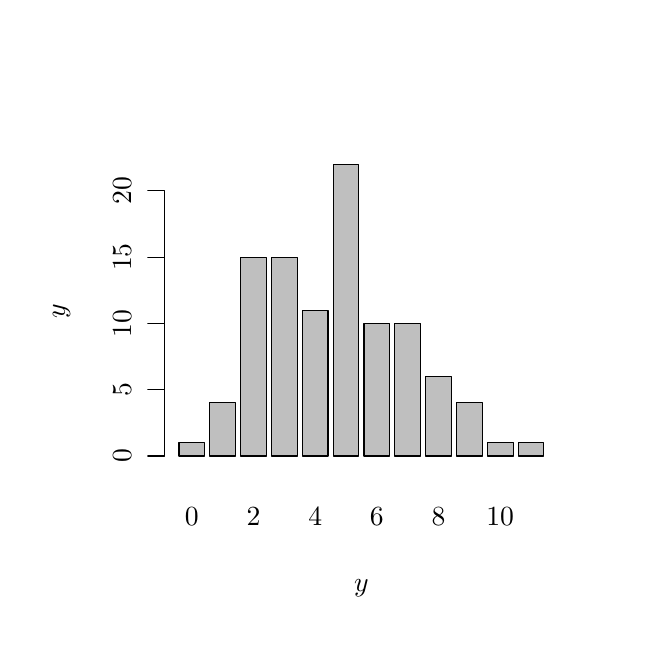
\begin{tikzpicture}[x=1pt,y=1pt]
\draw[color=white,opacity=0] (0,0) rectangle (216.81,216.81);
\begin{scope}
\path[clip] (  0.00,  0.00) rectangle (216.81,216.81);
\definecolor[named]{drawColor}{rgb}{0.88,0.97,0.36}
\definecolor[named]{drawColor}{rgb}{0.00,0.00,0.00}
\definecolor[named]{fillColor}{rgb}{0.75,0.75,0.75}

\draw[color=drawColor,line cap=round,line join=round,fill=fillColor,] ( 54.47, 62.25) rectangle ( 63.76, 67.04);

\draw[color=drawColor,line cap=round,line join=round,fill=fillColor,] ( 65.62, 62.25) rectangle ( 74.90, 81.41);

\draw[color=drawColor,line cap=round,line join=round,fill=fillColor,] ( 76.76, 62.25) rectangle ( 86.05,134.09);

\draw[color=drawColor,line cap=round,line join=round,fill=fillColor,] ( 87.90, 62.25) rectangle ( 97.19,134.09);

\draw[color=drawColor,line cap=round,line join=round,fill=fillColor,] ( 99.05, 62.25) rectangle (108.33,114.93);

\draw[color=drawColor,line cap=round,line join=round,fill=fillColor,] (110.19, 62.25) rectangle (119.48,167.61);

\draw[color=drawColor,line cap=round,line join=round,fill=fillColor,] (121.33, 62.25) rectangle (130.62,110.14);

\draw[color=drawColor,line cap=round,line join=round,fill=fillColor,] (132.48, 62.25) rectangle (141.76,110.14);

\draw[color=drawColor,line cap=round,line join=round,fill=fillColor,] (143.62, 62.25) rectangle (152.91, 90.99);

\draw[color=drawColor,line cap=round,line join=round,fill=fillColor,] (154.76, 62.25) rectangle (164.05, 81.41);

\draw[color=drawColor,line cap=round,line join=round,fill=fillColor,] (165.91, 62.25) rectangle (175.19, 67.04);

\draw[color=drawColor,line cap=round,line join=round,fill=fillColor,] (177.05, 62.25) rectangle (186.34, 67.04);
\end{scope}
\begin{scope}
\path[clip] (  0.00,  0.00) rectangle (216.81,216.81);
\definecolor[named]{drawColor}{rgb}{0.88,0.97,0.36}
\definecolor[named]{drawColor}{rgb}{0.00,0.00,0.00}

\node[color=drawColor,anchor=base,inner sep=0pt, outer sep=0pt, scale=  1.00] at ( 59.12, 37.20) {0%
};

\node[color=drawColor,anchor=base,inner sep=0pt, outer sep=0pt, scale=  1.00] at ( 81.40, 37.20) {2%
};

\node[color=drawColor,anchor=base,inner sep=0pt, outer sep=0pt, scale=  1.00] at (103.69, 37.20) {4%
};

\node[color=drawColor,anchor=base,inner sep=0pt, outer sep=0pt, scale=  1.00] at (125.98, 37.20) {6%
};

\node[color=drawColor,anchor=base,inner sep=0pt, outer sep=0pt, scale=  1.00] at (148.26, 37.20) {8%
};

\node[color=drawColor,anchor=base,inner sep=0pt, outer sep=0pt, scale=  1.00] at (170.55, 37.20) {10%
};
\end{scope}
\begin{scope}
\path[clip] (  0.00,  0.00) rectangle (216.81,216.81);
\definecolor[named]{drawColor}{rgb}{0.88,0.97,0.36}
\definecolor[named]{drawColor}{rgb}{0.00,0.00,0.00}

\node[color=drawColor,anchor=base,inner sep=0pt, outer sep=0pt, scale=  1.00] at (120.41, 13.20) {$y$
};

\node[rotate= 90.00,color=drawColor,anchor=base,inner sep=0pt, outer sep=0pt, scale=  1.00] at ( 13.20,114.41) {$\Prob{y}$
};
\end{scope}
\begin{scope}
\path[clip] (  0.00,  0.00) rectangle (216.81,216.81);
\definecolor[named]{drawColor}{rgb}{0.88,0.97,0.36}
\definecolor[named]{drawColor}{rgb}{0.00,0.00,0.00}

\draw[color=drawColor,line cap=round,line join=round,fill opacity=0.00,] ( 49.20, 62.25) -- ( 49.20,158.03);

\draw[color=drawColor,line cap=round,line join=round,fill opacity=0.00,] ( 49.20, 62.25) -- ( 43.20, 62.25);

\draw[color=drawColor,line cap=round,line join=round,fill opacity=0.00,] ( 49.20, 86.20) -- ( 43.20, 86.20);

\draw[color=drawColor,line cap=round,line join=round,fill opacity=0.00,] ( 49.20,110.14) -- ( 43.20,110.14);

\draw[color=drawColor,line cap=round,line join=round,fill opacity=0.00,] ( 49.20,134.09) -- ( 43.20,134.09);

\draw[color=drawColor,line cap=round,line join=round,fill opacity=0.00,] ( 49.20,158.03) -- ( 43.20,158.03);

\node[rotate= 90.00,color=drawColor,anchor=base,inner sep=0pt, outer sep=0pt, scale=  1.00] at ( 37.20, 62.25) {0%
};

\node[rotate= 90.00,color=drawColor,anchor=base,inner sep=0pt, outer sep=0pt, scale=  1.00] at ( 37.20, 86.20) {5%
};

\node[rotate= 90.00,color=drawColor,anchor=base,inner sep=0pt, outer sep=0pt, scale=  1.00] at ( 37.20,110.14) {10%
};

\node[rotate= 90.00,color=drawColor,anchor=base,inner sep=0pt, outer sep=0pt, scale=  1.00] at ( 37.20,134.09) {15%
};

\node[rotate= 90.00,color=drawColor,anchor=base,inner sep=0pt, outer sep=0pt, scale=  1.00] at ( 37.20,158.03) {20%
};
\end{scope}
\end{tikzpicture}

	\end{center}
	\end{frame}


	\begin{frame}
	\frametitle{Zero-Inflated Poisson Distribution}
	\noindent A sample from a Zero-inflated Poisson model, with Poisson distribution component with $\lambda=5$, and probability of zero-model being $.25$.
	\vspace{-2\baselineskip}
	\begin{center}
	
% Created by tikzDevice version 0.5.3 on 2011-03-10 21:35:39
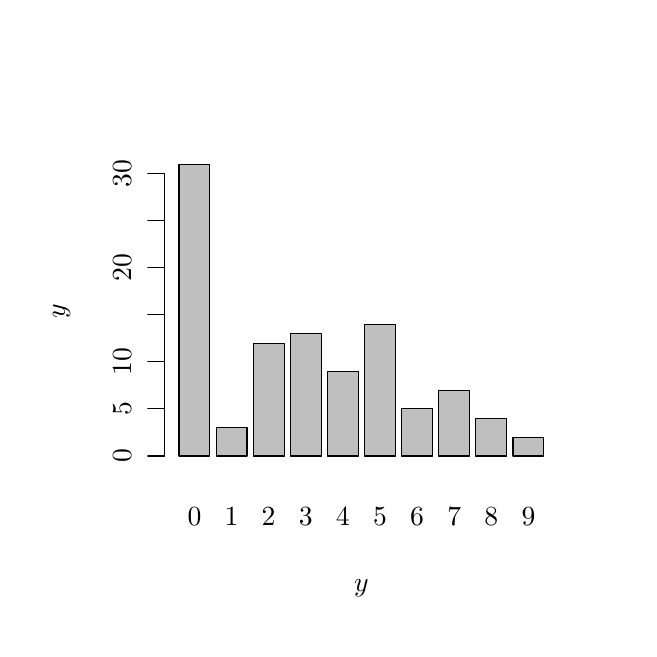
\begin{tikzpicture}[x=1pt,y=1pt]
\draw[color=white,opacity=0] (0,0) rectangle (216.81,216.81);
\begin{scope}
\path[clip] (  0.00,  0.00) rectangle (216.81,216.81);
\definecolor[named]{drawColor}{rgb}{0.50,0.23,0.81}
\definecolor[named]{drawColor}{rgb}{0.00,0.00,0.00}
\definecolor[named]{fillColor}{rgb}{0.75,0.75,0.75}

\draw[color=drawColor,line cap=round,line join=round,fill=fillColor,] ( 54.47, 62.25) rectangle ( 65.65,167.61);

\draw[color=drawColor,line cap=round,line join=round,fill=fillColor,] ( 67.88, 62.25) rectangle ( 79.06, 72.45);

\draw[color=drawColor,line cap=round,line join=round,fill=fillColor,] ( 81.29, 62.25) rectangle ( 92.47,103.04);

\draw[color=drawColor,line cap=round,line join=round,fill=fillColor,] ( 94.70, 62.25) rectangle (105.88,106.44);

\draw[color=drawColor,line cap=round,line join=round,fill=fillColor,] (108.11, 62.25) rectangle (119.29, 92.84);

\draw[color=drawColor,line cap=round,line join=round,fill=fillColor,] (121.52, 62.25) rectangle (132.70,109.83);

\draw[color=drawColor,line cap=round,line join=round,fill=fillColor,] (134.93, 62.25) rectangle (146.11, 79.25);

\draw[color=drawColor,line cap=round,line join=round,fill=fillColor,] (148.34, 62.25) rectangle (159.52, 86.04);

\draw[color=drawColor,line cap=round,line join=round,fill=fillColor,] (161.75, 62.25) rectangle (172.93, 75.85);

\draw[color=drawColor,line cap=round,line join=round,fill=fillColor,] (175.16, 62.25) rectangle (186.34, 69.05);
\end{scope}
\begin{scope}
\path[clip] (  0.00,  0.00) rectangle (216.81,216.81);
\definecolor[named]{drawColor}{rgb}{0.50,0.23,0.81}
\definecolor[named]{drawColor}{rgb}{0.00,0.00,0.00}

\node[color=drawColor,anchor=base,inner sep=0pt, outer sep=0pt, scale=  1.00] at ( 60.06, 37.20) {0%
};

\node[color=drawColor,anchor=base,inner sep=0pt, outer sep=0pt, scale=  1.00] at ( 73.47, 37.20) {1%
};

\node[color=drawColor,anchor=base,inner sep=0pt, outer sep=0pt, scale=  1.00] at ( 86.88, 37.20) {2%
};

\node[color=drawColor,anchor=base,inner sep=0pt, outer sep=0pt, scale=  1.00] at (100.29, 37.20) {3%
};

\node[color=drawColor,anchor=base,inner sep=0pt, outer sep=0pt, scale=  1.00] at (113.70, 37.20) {4%
};

\node[color=drawColor,anchor=base,inner sep=0pt, outer sep=0pt, scale=  1.00] at (127.11, 37.20) {5%
};

\node[color=drawColor,anchor=base,inner sep=0pt, outer sep=0pt, scale=  1.00] at (140.52, 37.20) {6%
};

\node[color=drawColor,anchor=base,inner sep=0pt, outer sep=0pt, scale=  1.00] at (153.93, 37.20) {7%
};

\node[color=drawColor,anchor=base,inner sep=0pt, outer sep=0pt, scale=  1.00] at (167.34, 37.20) {8%
};

\node[color=drawColor,anchor=base,inner sep=0pt, outer sep=0pt, scale=  1.00] at (180.75, 37.20) {9%
};
\end{scope}
\begin{scope}
\path[clip] (  0.00,  0.00) rectangle (216.81,216.81);
\definecolor[named]{drawColor}{rgb}{0.50,0.23,0.81}
\definecolor[named]{drawColor}{rgb}{0.00,0.00,0.00}

\node[color=drawColor,anchor=base,inner sep=0pt, outer sep=0pt, scale=  1.00] at (120.41, 13.20) {$y$
};

\node[rotate= 90.00,color=drawColor,anchor=base,inner sep=0pt, outer sep=0pt, scale=  1.00] at ( 13.20,114.41) {$\Prob{y}$
};
\end{scope}
\begin{scope}
\path[clip] (  0.00,  0.00) rectangle (216.81,216.81);
\definecolor[named]{drawColor}{rgb}{0.50,0.23,0.81}
\definecolor[named]{drawColor}{rgb}{0.00,0.00,0.00}

\draw[color=drawColor,line cap=round,line join=round,fill opacity=0.00,] ( 49.20, 62.25) -- ( 49.20,164.21);

\draw[color=drawColor,line cap=round,line join=round,fill opacity=0.00,] ( 49.20, 62.25) -- ( 43.20, 62.25);

\draw[color=drawColor,line cap=round,line join=round,fill opacity=0.00,] ( 49.20, 79.25) -- ( 43.20, 79.25);

\draw[color=drawColor,line cap=round,line join=round,fill opacity=0.00,] ( 49.20, 96.24) -- ( 43.20, 96.24);

\draw[color=drawColor,line cap=round,line join=round,fill opacity=0.00,] ( 49.20,113.23) -- ( 43.20,113.23);

\draw[color=drawColor,line cap=round,line join=round,fill opacity=0.00,] ( 49.20,130.23) -- ( 43.20,130.23);

\draw[color=drawColor,line cap=round,line join=round,fill opacity=0.00,] ( 49.20,147.22) -- ( 43.20,147.22);

\draw[color=drawColor,line cap=round,line join=round,fill opacity=0.00,] ( 49.20,164.21) -- ( 43.20,164.21);

\node[rotate= 90.00,color=drawColor,anchor=base,inner sep=0pt, outer sep=0pt, scale=  1.00] at ( 37.20, 62.25) {0%
};

\node[rotate= 90.00,color=drawColor,anchor=base,inner sep=0pt, outer sep=0pt, scale=  1.00] at ( 37.20, 79.25) {5%
};

\node[rotate= 90.00,color=drawColor,anchor=base,inner sep=0pt, outer sep=0pt, scale=  1.00] at ( 37.20, 96.24) {10%
};

\node[rotate= 90.00,color=drawColor,anchor=base,inner sep=0pt, outer sep=0pt, scale=  1.00] at ( 37.20,130.23) {20%
};

\node[rotate= 90.00,color=drawColor,anchor=base,inner sep=0pt, outer sep=0pt, scale=  1.00] at ( 37.20,164.21) {30%
};
\end{scope}
\end{tikzpicture}

	\end{center}
	\end{frame}



\begin{frame}
	\frametitle{Dirichlet Process mixture models}
	\begin{itemize}
		\item Dirichlet Process mixture model can overcome the problem of choosing $K$, the number of component distributions.
		\item In a Dirichlet Process mixture model, our generative model is
		\\For $i \in \{1, 2 \ldots n\}$,
		\begin{align*}
			\theta_i &\sim \mathrm{DP}(\alpha G_0),\\
			y_i &\sim \Prob{y\given \theta_i}
		\end{align*}
		which is equivalent to 
		\[
			\Prob{y_i} \sim \sum_{k=1}^\infty \Prob{y \given \theta, x_i=k}\Prob{x_i=k\given\pi}, \quad\text{for $i \in {1 \ldots n}$.}
		\]
	

	\end{itemize}
\end{frame}


\begin{frame}
	\frametitle{Dirichlet Process mixture models}
	\begin{itemize}
		\item A Dirichlet Process with \emph{base measure} $G_0$ and \emph{concentration} parameter $\alpha$ can be defined by followng density:
			\[
				f(\theta) = \sum_{k=1}^\infty \pi_k \delta_{\theta_k}(\theta)
			\]
			where each $\pi_k$ is drawn from a \emph{stick-breaking} prior with parameter $\alpha$, each $\theta_k$ is drawn $G_0$, and 
		\[
			\delta_{\theta_k}(\theta)
		\]
		is an function over $\theta$ that takes the value of $1$ if $\theta=\theta_k$ and $0$ otherwise.
		\item In other words, a Dirchlet Process $f(\theta)$ is an infinite distribution of \emph{spikes} on the $\theta$ parameter space.


	\end{itemize}
\end{frame}



\end{document}
